\documentclass{article}
\usepackage{CJK}
\usepackage{graphicx}
\usepackage{geometry}

\begin{document}
\newgeometry{layout=a4paper}
\begin{CJK*}{GBK}{song}
\title{\textbf{北京市气象数据可视化\\实验报告}}
\author{A \and{000}\and{  B}\and{ 001}}
\maketitle

\section{实验目标}
\qquad 自2013年北京第一次出现雾霾以来,北京的空气质量备受世人关注,同时也是关乎每位老师同学身心健康的大事。近年来,北京不断添加空气质量监测设备、不断完善数据公开制度,让每位市民都能实时了解到北京天气如何。

%%%%%%%%%%%%%%%%%%%%%%%%%%%%%%%%%% 修改段落间距: \setlength{\parskip}{0pt} 用弹性距离;
%%%%%%%%%%%%%%%%%%%%%%%%%%%%%%%%%% 修改行间距是:\setlength{\baselineskip}{1.5\baselineskip} 或者 \setlength{\baselineskip}{20pt}
\setlength{\parskip}{10pt}时间已经过去了将近两年,数据也已经积累了很多,但是大多数人也还是停留在翻看一下今天的PM2.5是多少的习惯上,很少见到有人对历史数据进行研究整理。所以想借本课程的机会,研究一下北京的空气质量数据。

北京空气质量由北京市环境保护监测中心负责,通过北京各区县设立的35个监测站进行实时测量。目前收集的空气质量数据包括:$PM2.5$、$PM10$、$AQI$、$SO_2$、$NO_2$、$O_3$、$CO$ 每小时一次的实际值以及它们各自在过去24小时的平均值,共计14个指标。本方案就是针对这些数据进行可视化分析。

我们的研究目标整体上分三层:\\
1、对官方数据进行清洗并存储;\\
2、任意数据的精确查询,并实现任意时点数据的可视化、任意时间段数据的动态展示;\\
3、在此基础上进行空气质量变化规律的分析。

\section{数据介绍}
\qquad 北京空气质量可以实时地通过http://zx.bjmemc.com.cn/网站查看,但是该网站并不负责提供历史数据,所以需要自行抓取数据。
网站提供的数据包括从20131205至今的每小时测量一次的污染物浓度数据。已经拿到的数据格式是:

\begin{figure}[ht]
\centering
\scalebox{0.7}{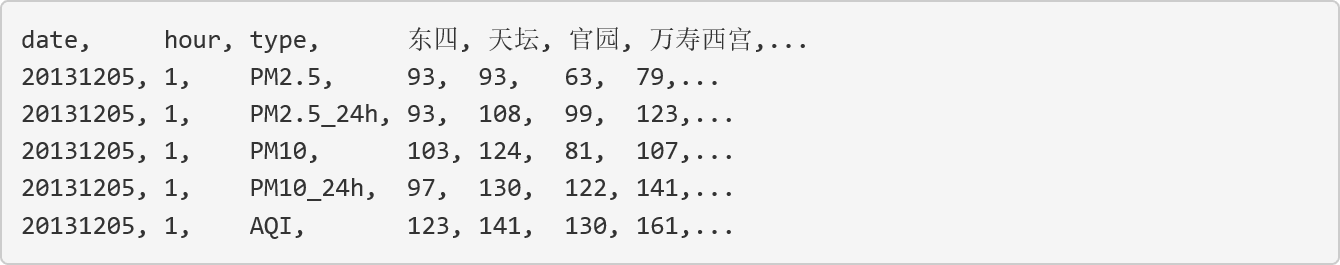
\includegraphics{1.png}}
\caption{\textit{已获取的数据格式}}
\end{figure}

数据含义是:
\begin{center}
\begin{tabular}{|c|c|c|} \hline
\textbf{Type} & \textbf{数据类型} & \textbf{单位} \\ \hline
PM2.5 & PM2.5实时浓度 & (微克/立方米) \\ \hline
PM2.5\_24h & PM2.5 24小时均值 & (微克/立方米) \\ \hline
PM10 & PM10实时浓度 & (微克/立方米) \\ \hline
PM10\_24h & PM10 24小时均值 & (微克/立方米) \\ \hline
AQI & AQI实时值 & N/A \\ \hline
SO2 & SO2实时浓度 & (微克/立方米) \\ \hline
SO2\_24h & SO2 24小时均值 & (微克/立方米) \\ \hline
NO2 & NO2实时浓度 & (微克/立方米) \\ \hline
NO2\_24h & NO2 24小时均值 & (微克/立方米) \\ \hline
O3 & O3实时浓度 & (微克/立方米) \\ \hline
CO & CO实时浓度 & (毫克/立方米) \\ \hline
CO\_24h & CO 24小时均值 & (毫克/立方米) \\ \hline
\end{tabular}
\end{center}

北京市共35个监测站,涵盖所有的16个区县,每个区县最多3个,最少1个。35个监测站的地理位置与详细信息是:

\begin{figure}[ht]
\centering
\scalebox{0.18}{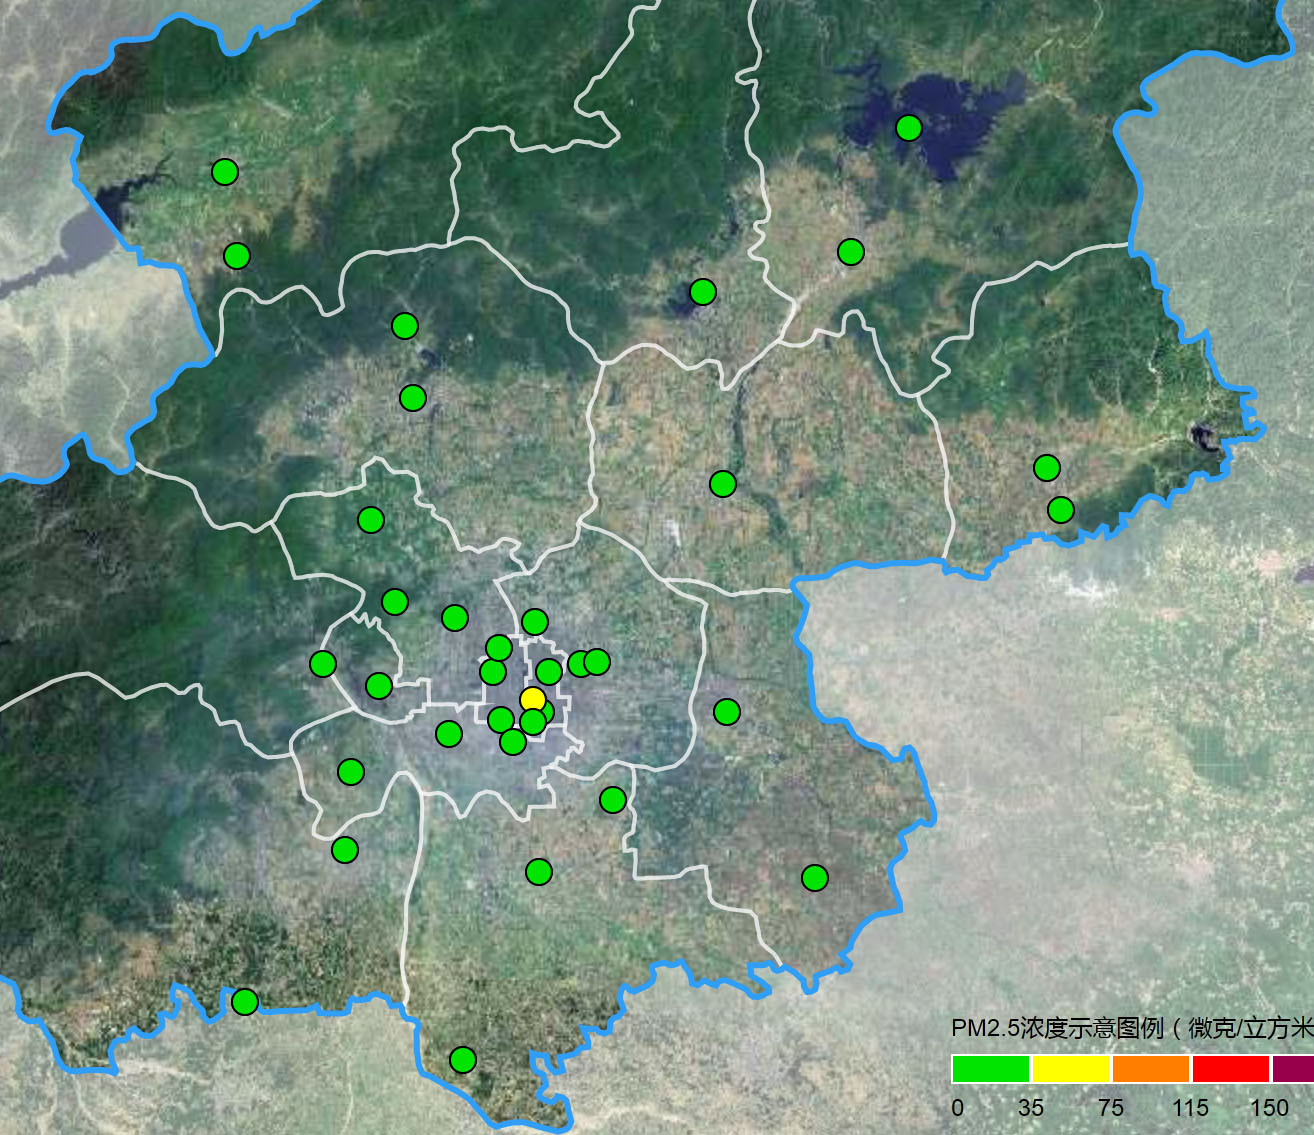
\includegraphics{2.jpg}}
\caption{\textit{35个监测站的位置}}
\end{figure}


\begin{center}
\begin{tabular}{|c|c|c|c|} \hline
\multicolumn{4}{|c|}{\textbf{城区环境评价点12个}} \\ \hline
\textbf{监测点} & \textbf{监测点全称} & \textbf{经度} & \textbf{纬度} \\ \hline
东四 & 东城东四 & 116.417 & 39.929 \\ \hline
天坛 & 东城天坛 & 116.407 & 39.886 \\ \hline
官园 & 西城官园 & 116.339 & 39.929 \\ \hline
万寿西宫 & 西城万寿西宫 & 116.352 & 39.878 \\ \hline
奥体中心 & 朝阳奥体中心 & 116.397 & 39.982 \\ \hline
农展馆 & 朝阳农展馆 & 116.461 & 39.937 \\ \hline
万柳 & 海淀万柳 & 116.287 & 39.987 \\ \hline
北部新区 & 海淀北部新区 & 116.174 & 40.09 \\ \hline
植物园 & 海淀北京植物园 & 116.207 & 40.002 \\ \hline
丰台花园 & 丰台花园 & 116.279 & 39.863 \\ \hline
云岗 & 丰台云岗 & 116.146 & 39.824 \\ \hline
古城 & 石景山古城 & 116.184 & 39.914 \\ \hline
\end{tabular}


\quad \\
%%%%%%%%%%%%%%%%%%%%%%%%%%%%%%%%%%% 输入\比较麻烦:$\backslash$

\begin{tabular}{|c|c|c|c|} \hline
\multicolumn{4}{|c|}{\textbf{郊区环境评价点11个}} \\ \hline
\textbf{监测点} & \textbf{监测点全称} & \textbf{经度} & \textbf{纬度} \\ \hline
房山 & 房山良乡 & 116.136 & 39.742 \\ \hline
大兴 & 大兴黄村镇 & 116.404 & 39.718 \\ \hline
亦庄 & 亦庄开发区 & 116.506 & 39.795 \\ \hline
通州 & 通州新城 & 116.663 & 39.886 \\ \hline
顺义 & 顺义新城 & 116.655 & 40.127 \\ \hline
昌平 & 昌平镇 & 116.23 & 40.217 \\ \hline
门头沟 & 门头沟龙泉镇 & 116.106 & 39.937 \\ \hline
平谷 & 平谷镇 & 117.1 & 40.143 \\ \hline
怀柔 & 怀柔镇 & 116.628 & 40.328 \\ \hline
密云 & 密云镇 & 116.832 & 40.37 \\ \hline
延庆 & 延庆镇 & 115.972 & 40.453 \\ \hline
\end{tabular}

\begin{tabular}{|c|c|c|c|} \hline
\multicolumn{4}{|c|}{\textbf{对照点及区域点7个}} \\ \hline
\textbf{监测点} & \textbf{监测点全称} & \textbf{经度} & \textbf{纬度} \\ \hline
定陵 & 昌平定陵 & 116.22 & 40.292 \\ \hline
八达岭 & 京西北八达岭 & 115.988 & 40.365 \\ \hline
密云水库 & 京东北密云水库 & 116.911 & 40.499 \\ \hline
东高村 & 京东东高村 & 117.12 & 40.10 \\ \hline
永乐店 & 京东南永乐店 & 116.783 & 39.712 \\ \hline
榆垡 & 京南榆垡 & 116.30 & 39.52 \\ \hline
琉璃河 & 京西南琉璃河 & 116.00 & 39.58 \\ \hline
\end{tabular}

\begin{tabular}{|c|c|c|c|} \hline
\multicolumn{4}{|c|}{\textbf{交通污染监控点5个}} \\ \hline
\textbf{监测点} & \textbf{监测点全称} & \textbf{经度} & \textbf{纬度} \\ \hline
前门 & 前门东大街 & 116.395 & 39.899 \\ \hline
永定门内 & 永定门内大街 & 116.394 & 39.876 \\ \hline
西直门北 & 西直门北大街 & 116.349 & 39.954 \\ \hline
南三环 & 南三环西路 & 116.368 & 39.856 \\ \hline
东四环 & 东四环北路 & 116.483 & 39.939 \\ \hline
\end{tabular}
\end{center}


\section{可视化方案}
\qquad 使用百度地图API展示数据,最终以Web形式作为交互界面。Web包含四个页面:

\subsection{页面一:各区县污染物平均浓度展示}
\qquad 各区县内观测站数据求平均作为整个区县的数据,划分污染等级后用图层透明度展示污染物浓度。每个污染物根据《中国环境空气质量标准GB3095-1996》划分为6个等级,等级越低空气越好。具体如下:

\begin{center}
\begin{tabular}{|c|c|c|c|c|c|} \hline
污染物 & 等级1上限 & 等级2上限 & 等级3上限 & 等级4上限 & 等级5上限 \\ \hline
PM2.5 & 35 & 75 & 115 & 150 & 250 \\ \hline
PM10 & 50 & 150 & 250 & 350 & 420 \\ \hline
AQI & 50 & 100 & 150 & 200 & 300 \\ \hline
SO2 & 150 & 500 & 650 & 800 & 1600 \\ \hline
NO2 & 100 & 200 & 700 & 1200 & 2340 \\ \hline
O3 & 160 & 200 & 300 & 400 & 800 \\ \hline
CO & 5 & 10 & 35 & 60 & 90 \\ \hline
\end{tabular}
\end{center}

这个可视化视图下可以进行确定时间点的展示,也可以选择时间区间展示动画,效果如下:

\begin{figure}[ht]
\centering
\scalebox{0.35}{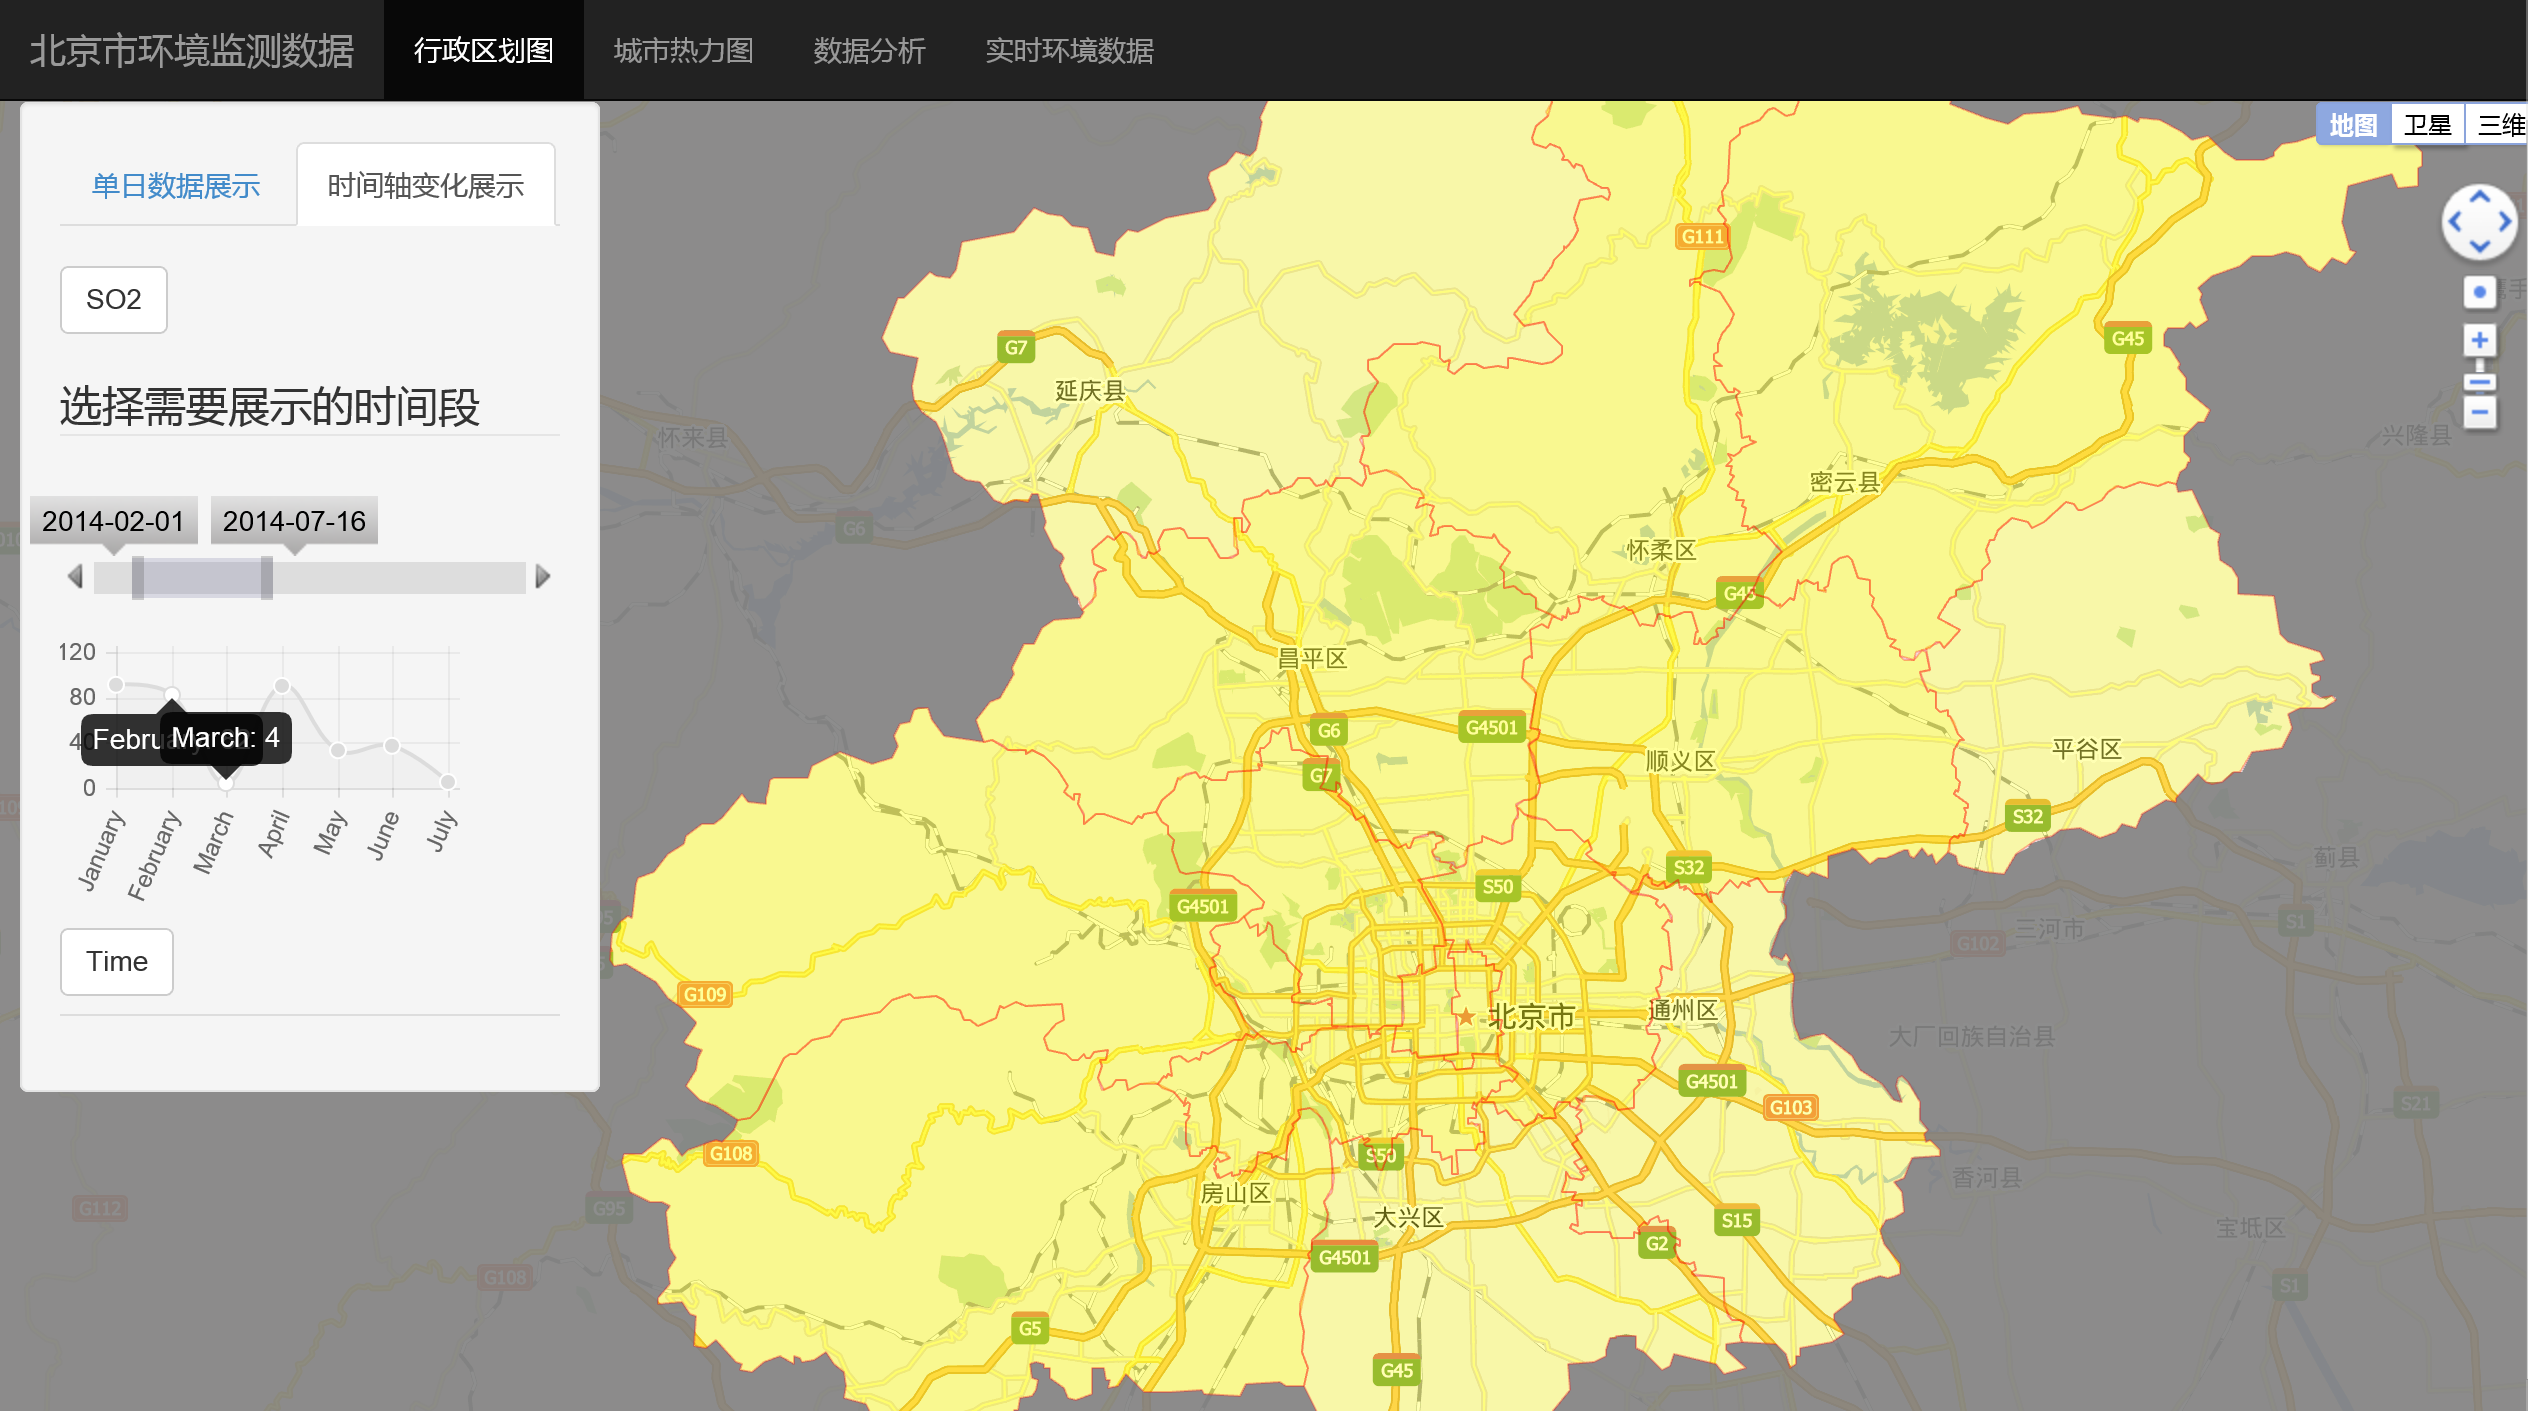
\includegraphics{3.png}}
\caption{\textit{页面一}}
\end{figure}

\subsection{页面二:各观测点污染物浓度热力图展示}
\qquad 各观测站数据直接做热力点,用点的大小和颜色一同展示浓度。该可视化视图下也可以进行确定时间点的展示,以及选择时间区间展示动画,效果如下:

\begin{figure}[ht]
\centering
\scalebox{0.35}{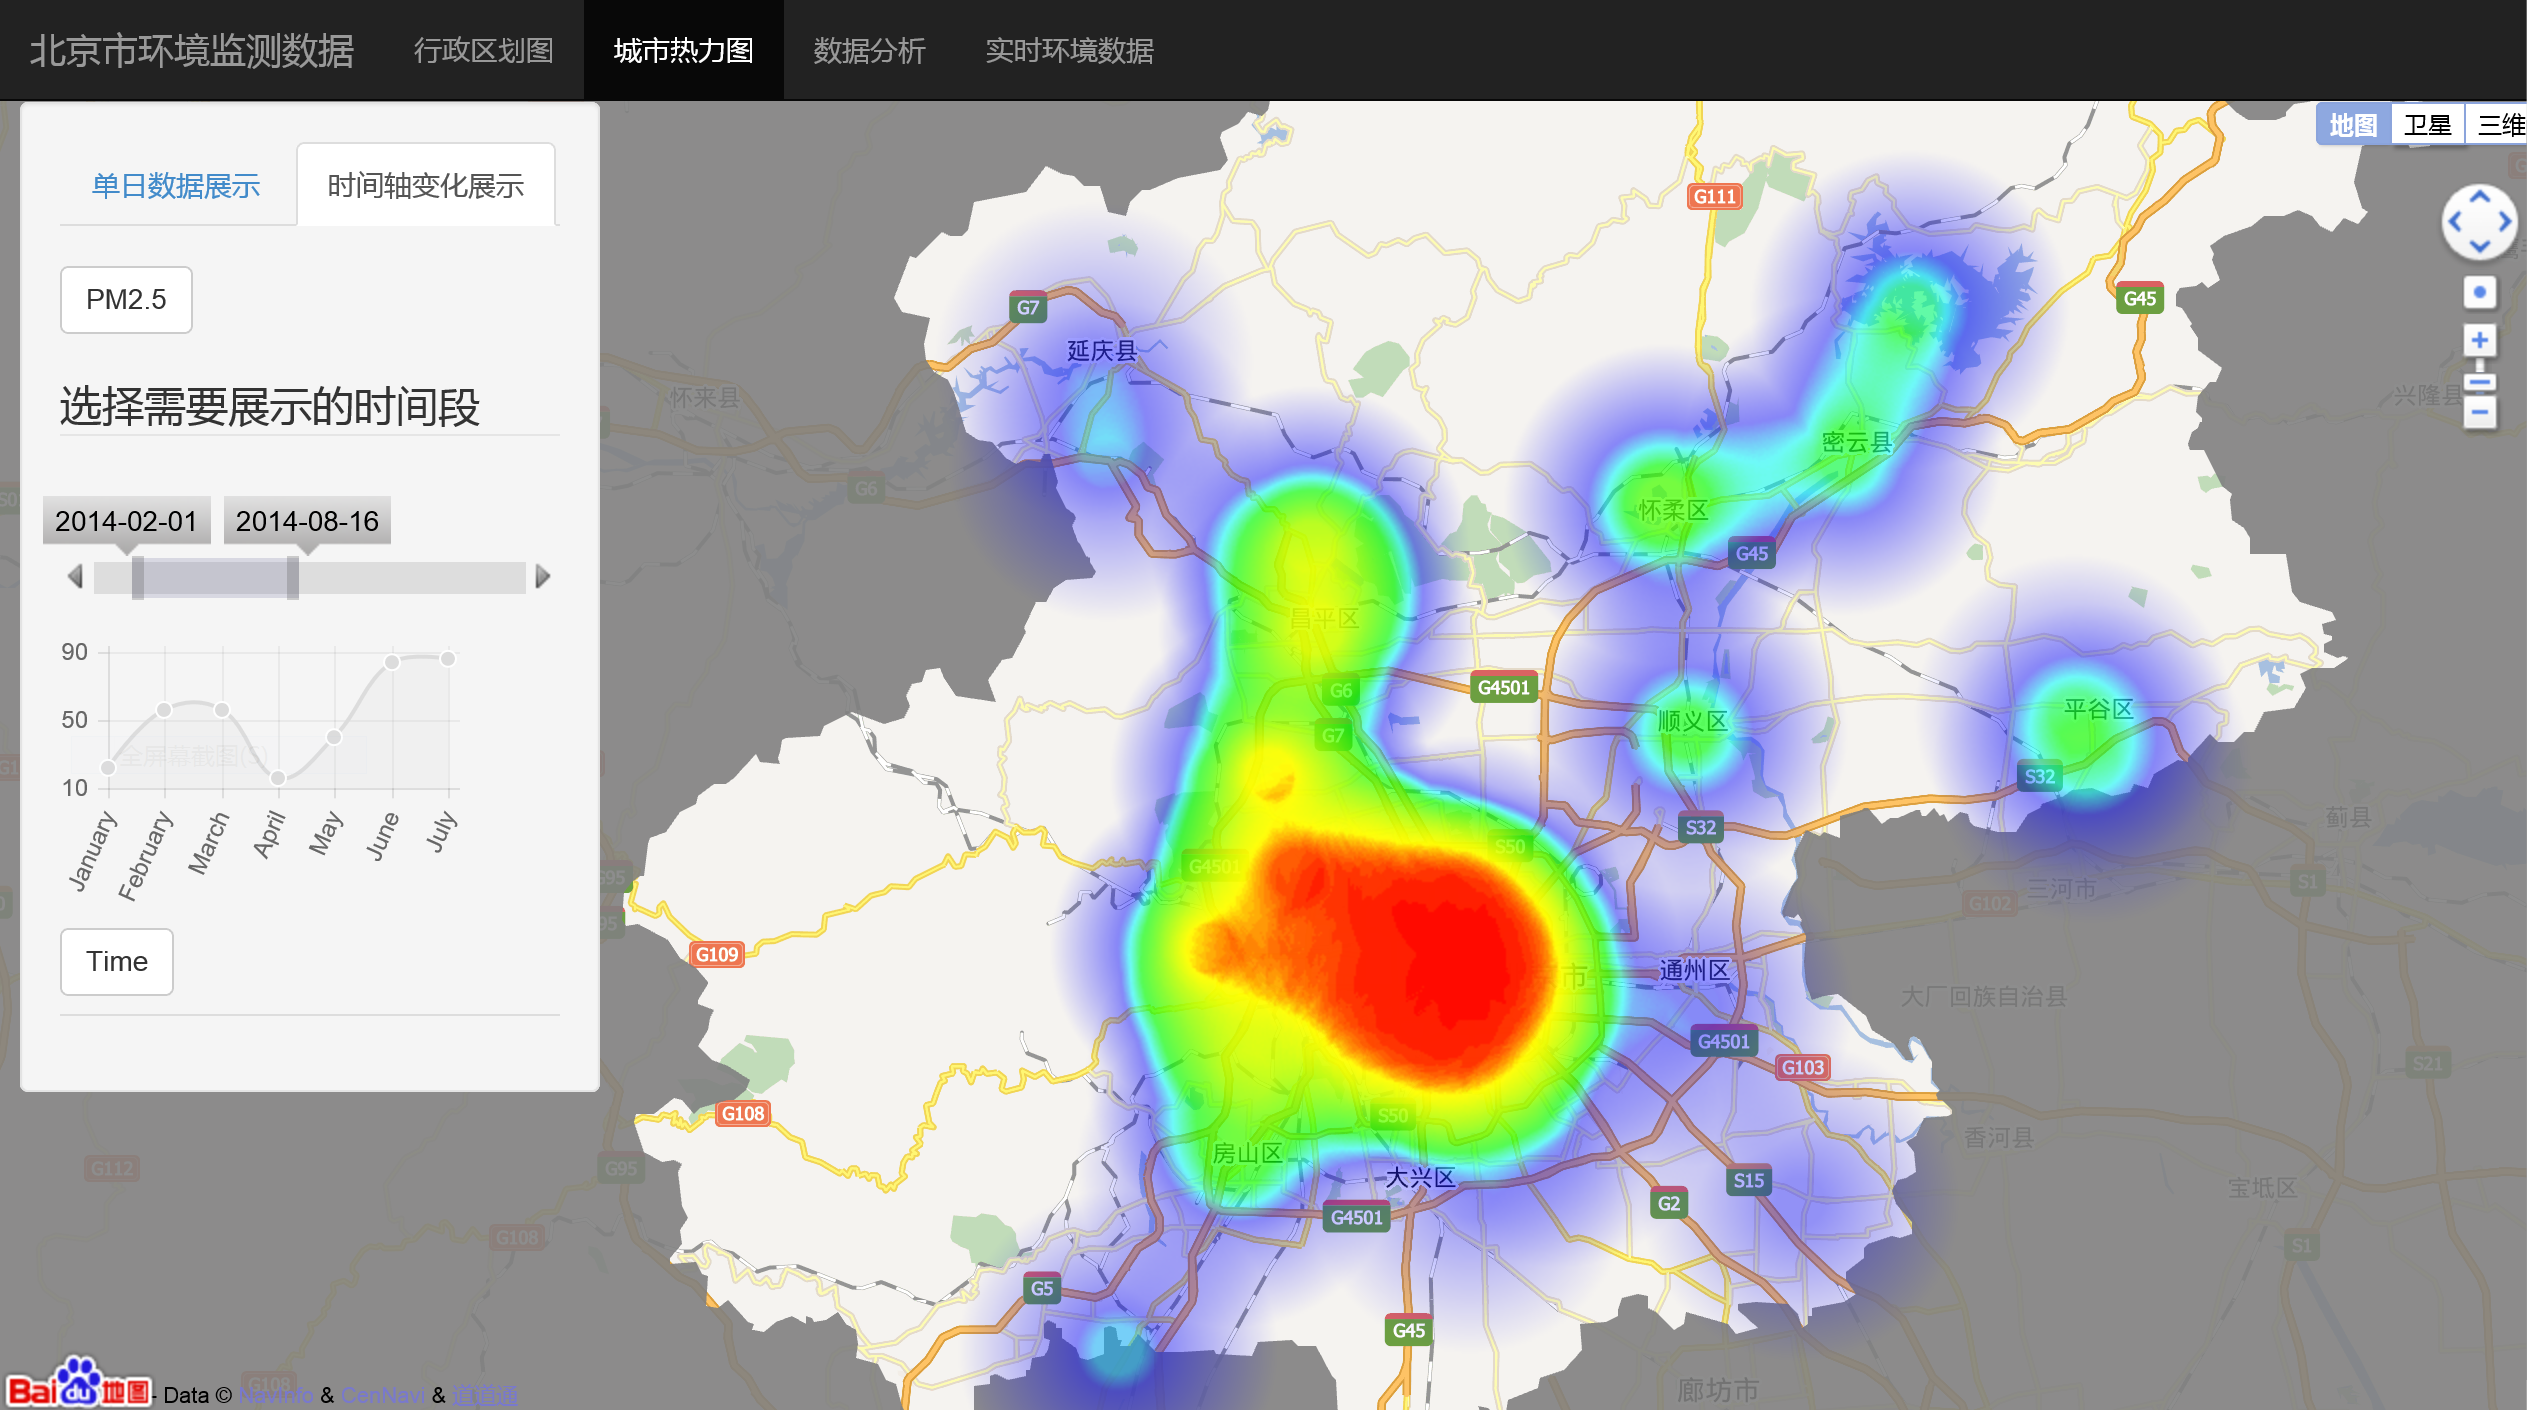
\includegraphics{4.png}}
\caption{\textit{页面二}}
\end{figure}


\subsection{页面三:统计分析}
\qquad 进行两种数据分析:单日24小时的7种污染物浓度曲线变化、任意时间段的某种确定污染物的浓度曲线变化。单日分析中需要指定确定的日期、确定的观测站;时间段的分析需要制定时间段、确定的污染物类型,效果如下:

\begin{figure}[ht]
\centering
\scalebox{0.35}{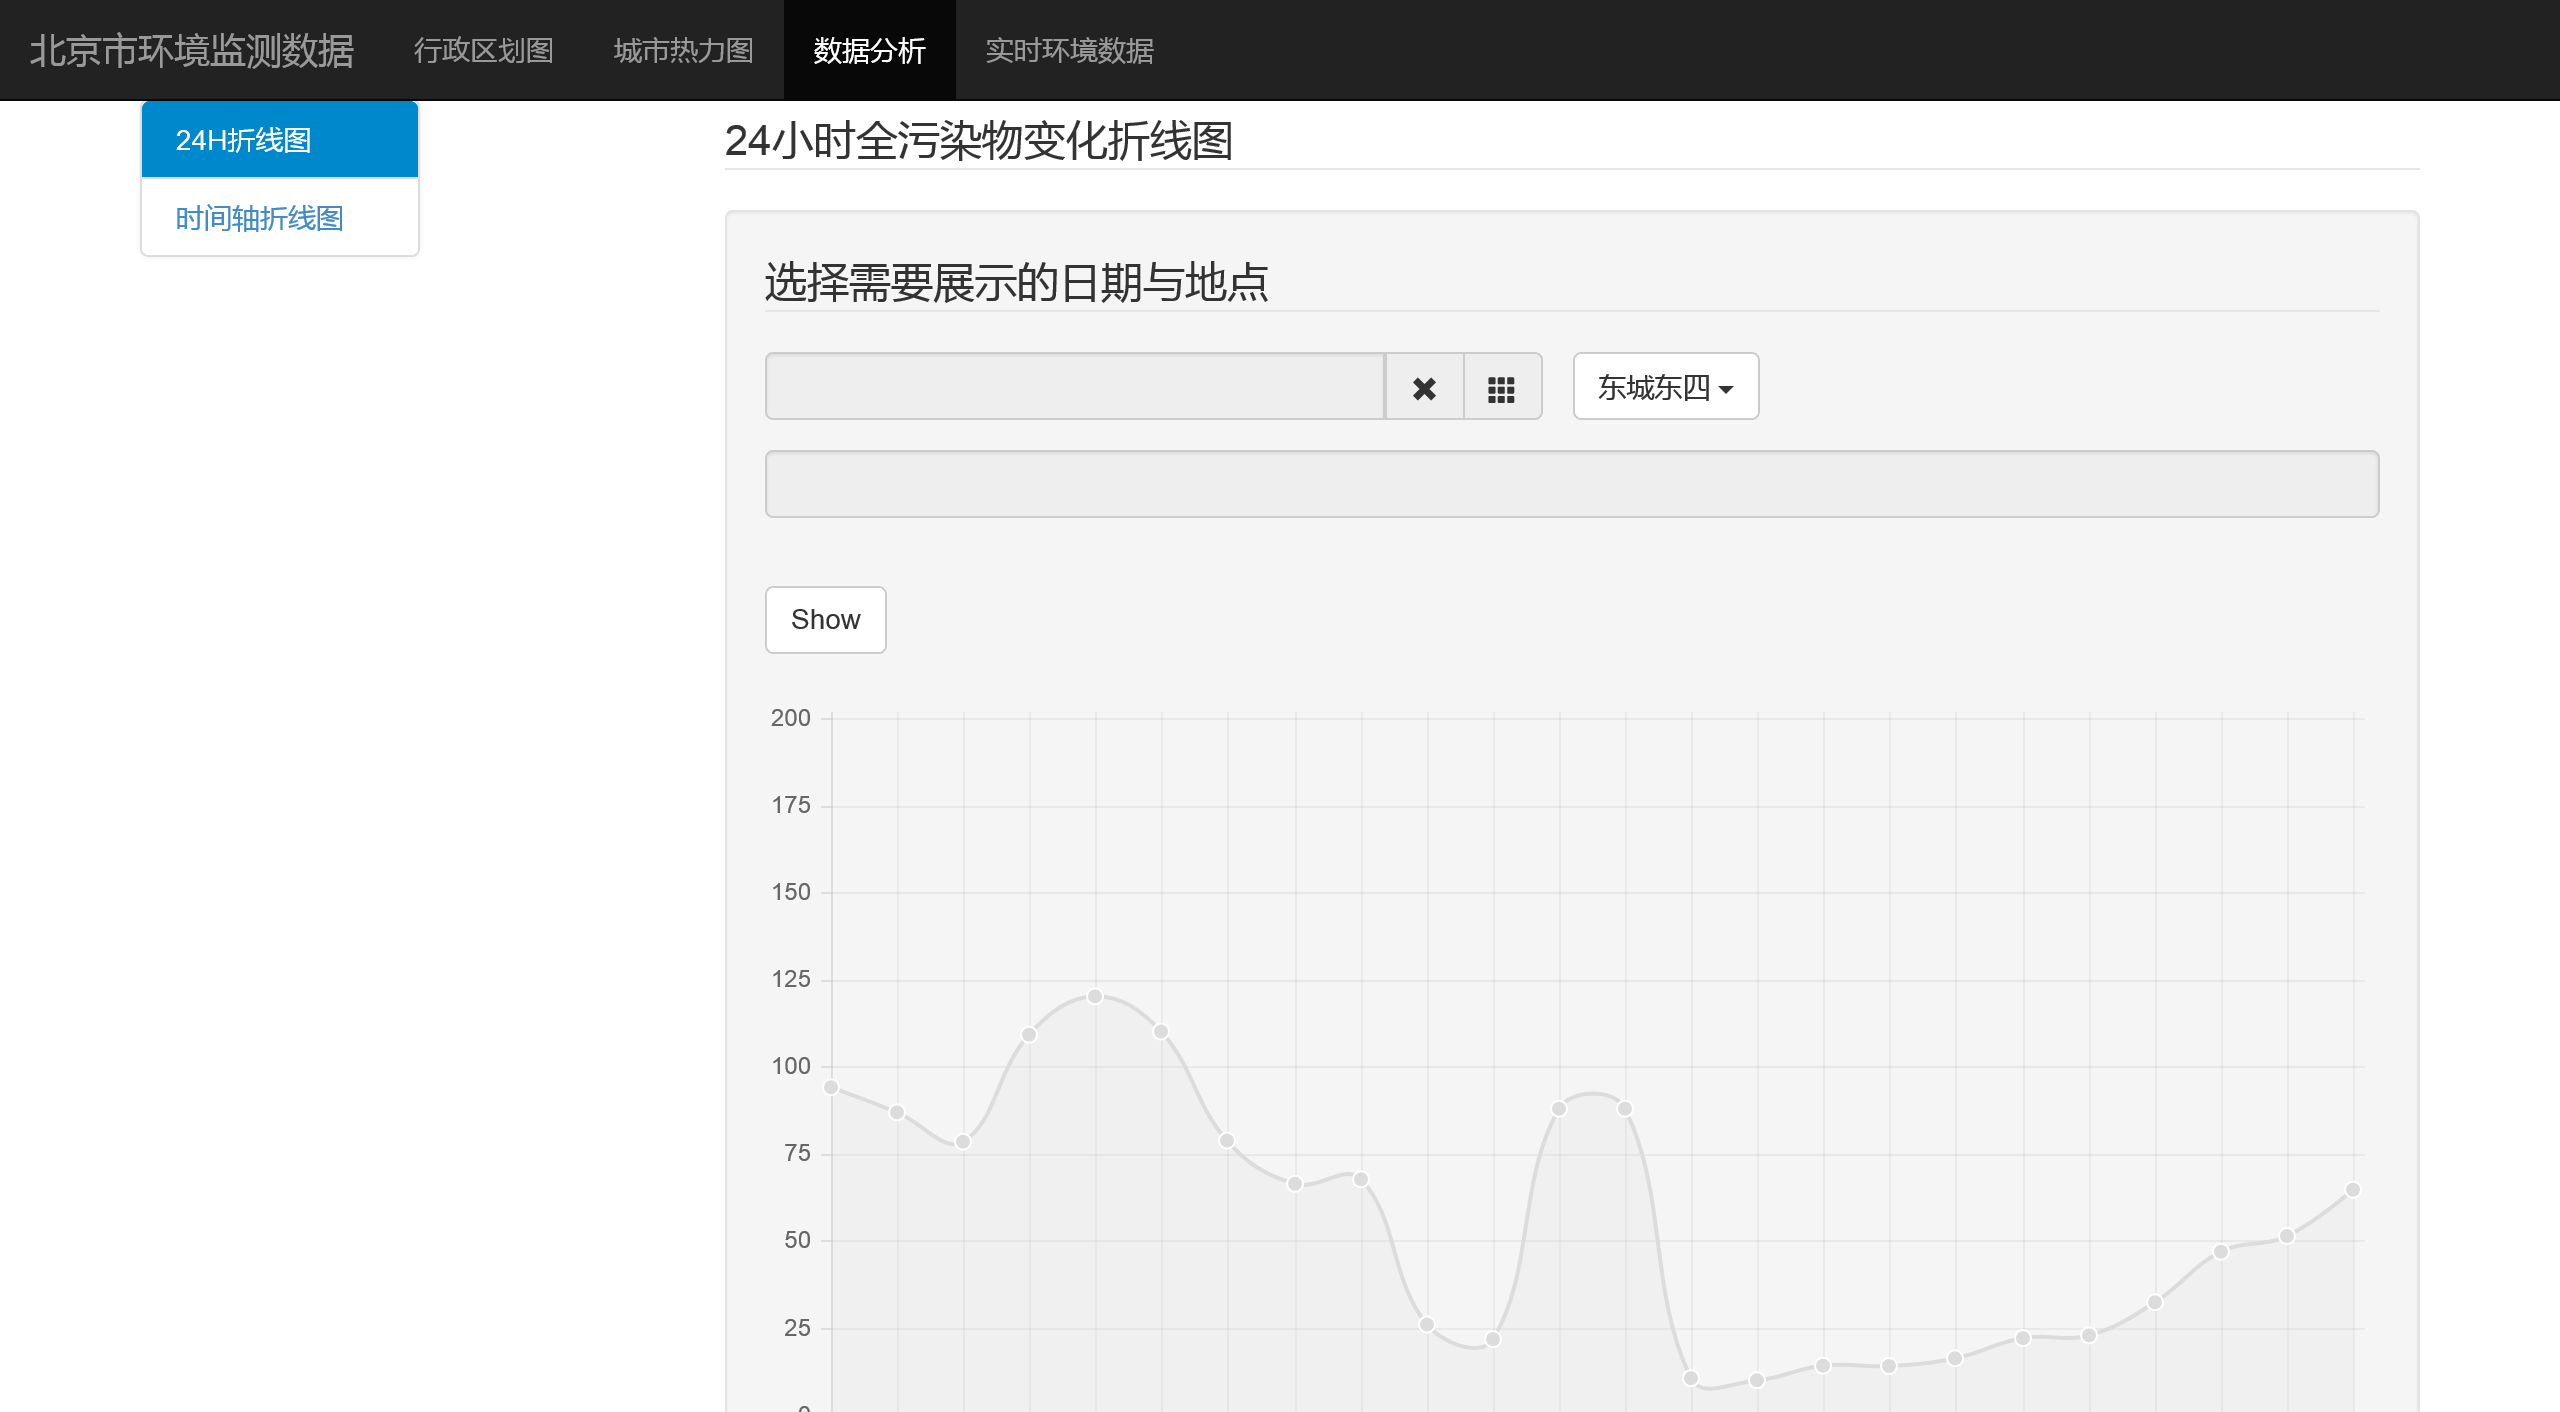
\includegraphics{5.png}}
\caption{\textit{页面三}}
\end{figure}

\subsection{页面四:精确数据查询}
\qquad 任意时间点、观测站、污染物类型的精确数据查询,除时间点外,均可以多选,效果如下:

\begin{figure}[ht]
\centering
\scalebox{0.35}{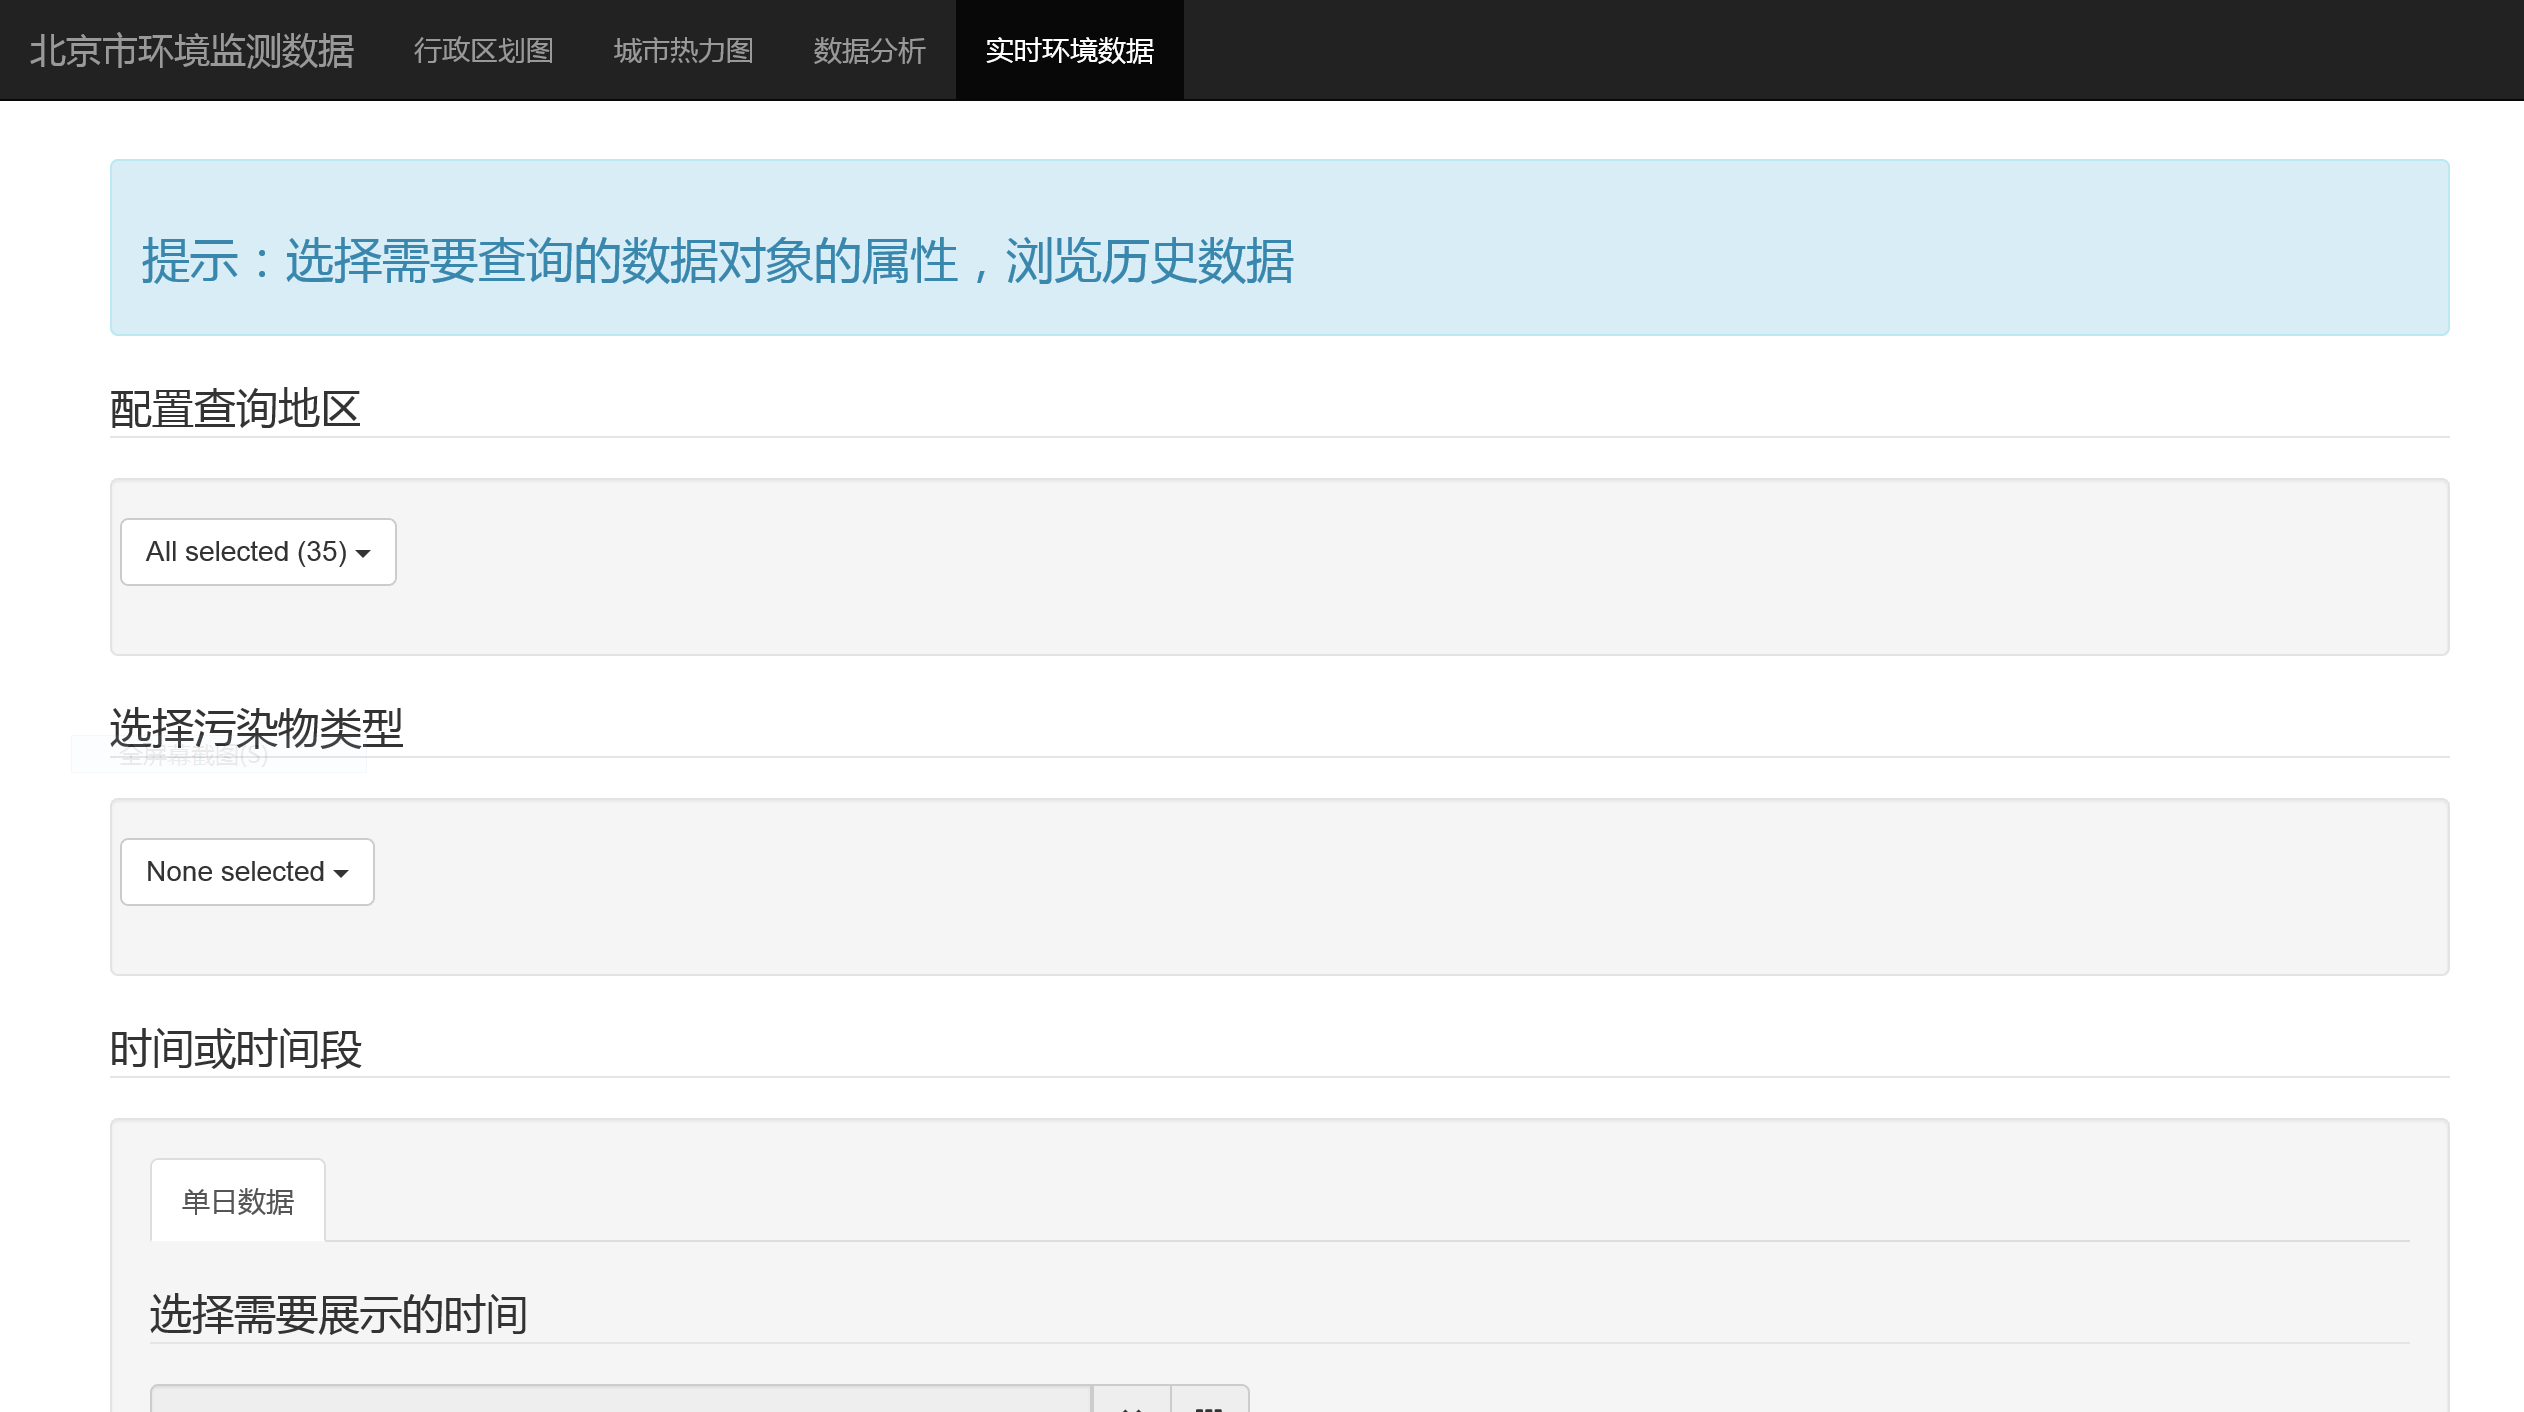
\includegraphics{6.png}}
\caption{\textit{页面四}}
\end{figure}


\section{可视化技术}

\subsection{数据清洗}
\qquad 项目建立的基础是北京市环境监测网站提供的数据文件,数据以.csv的形式保存。其格式为:

\begin{figure}[ht]
\centering
\scalebox{0.35}{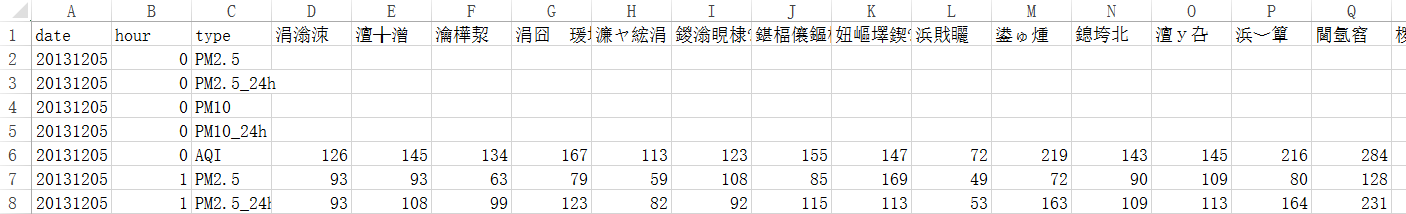
\includegraphics{H1.png}}
\end{figure}


数据的前3列分别存放对应日期、时间和污染物类型,之后的35列分别对应35个观测站。鉴于原始数据本身存在相当程度的缺失等异常情况,并存在一定程度的不合理数据,对于这些数据进行数据清洗工作存在其必要性。

首先是确定对于缺失数据和错误数据的修复策略。我们的选择是建立平均值矩阵,对应每一个观测站,每一种污染物,每一个时间段,建立对应的平均值矩阵,作为需要填充时的依据。

矩阵的部分结果为:

\begin{figure}[ht]
\centering
\scalebox{0.5}{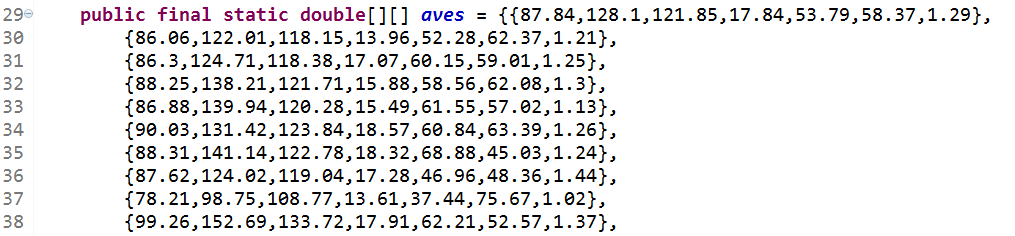
\includegraphics{H2.png}}
\end{figure}

对于异常数据,去除了数值异常大,明显不合理的数据,例如2013年底,50000数值的PM2.5指标等。


\subsection{数据库建设}

\qquad 本身采用.csv文件存储的环境监测数据集大约有21M左右,但是考虑到总共469天的检测区间,7中污染物,35个监测站,24小时的环境数据,一共会有24*35*7*469,大约2757720行的环境数据,单纯使用内存的方法,例如HashMap等难以满足复杂的查询需求,所以建立了数据库后台,用于支撑数据的相关操作。数据库使用MySQL进行建立,使用两张表来进行数据的存储。

imformation.bp\_position:存放监测站的地理位置等信息

\begin{figure}[ht]
\centering
\scalebox{0.5}{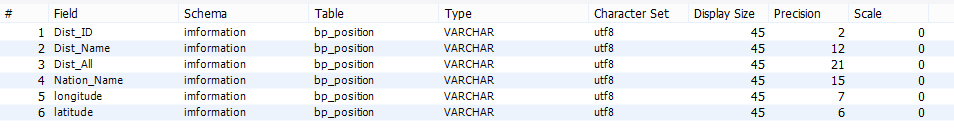
\includegraphics{H3.png}}
\end{figure}

imformation.bp\_data:存放具体的监测数据信息

\begin{figure}[ht]
\centering
\scalebox{0.5}{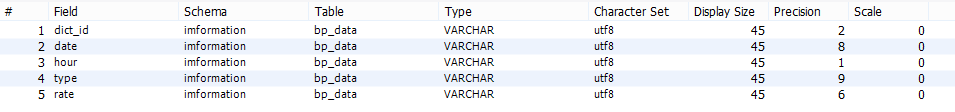
\includegraphics{H4.png}}
\end{figure}

使用这两张表将原始数据完成清洗之后的结果加以存储,完成数据的支撑工作。


\subsection{服务器搭建}

\qquad 鉴于我们的UI展示会采用网站的形式,需要完成服务器的搭建工作。服务器的构架是较为常用的Serverlet服务形式,使用Java语言完成后台处理代码的编写,并使用Jsp作为网页的编码形式,同时采用Tomcat作为网站的发布载体,完成网站服务器的搭建。

Serverlet结构截图:

\begin{figure}[ht]
\centering
\scalebox{0.7}{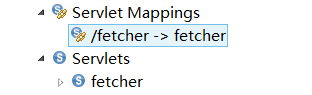
\includegraphics{H5.png}}
\end{figure}

Tomcat服务器运行截图:

\newpage

\begin{figure}[ht]
\centering
\scalebox{0.4}{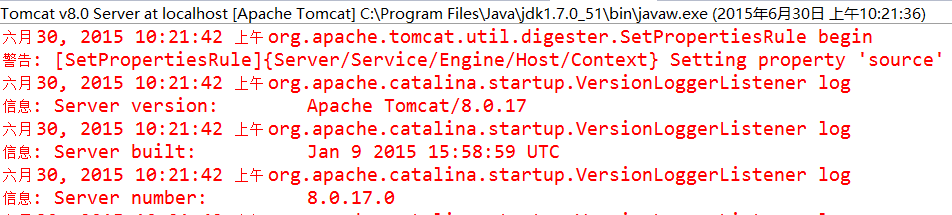
\includegraphics{H7.png}}
\end{figure}

\subsection{网站UI设计与实现}

\qquad 网页的UI采用了常用的Bootstrap项目结构,除了常规的Bootstrap和Jquery的相关内容之外,鉴于网站的内容,还采用了以下插件:\\
bootstrap-datetimepicker:提供日期的选择;\\
bootstrap-multiselect:提供条件复选;\\
bootstrap-table:提供表格的展示;\\
Chart.js:提供图标的展示;\\
jQRangeSlider:提供日期段的选取。

这些插件都存在于asset文件夹目录之下:

\begin{figure}[ht]
\centering
\scalebox{0.5}{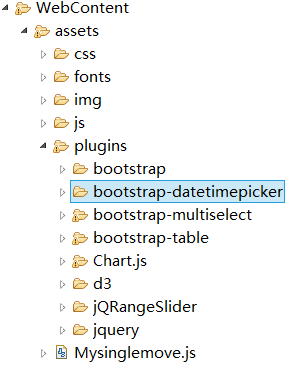
\includegraphics{H8.png}}
\end{figure}


\subsection{百度地图API}
\qquad 百度地图JavaScript API是一套由JavaScript语言编写的应用程序接口,可在网站中构建功能丰富、交互性强的地图应用,支持PC端和移动端基于浏览器的地图应用开发,且支持HTML5特性的地图开发。也是本次可视化中地图部分主要依赖的工具。

百度地图在中国有很好的链接速度,而且API完全免费、不限制使用次数,只需在developer.baidu.com上注册后,获得密钥即可。具体可见http://developer.baidu.com/map/index.php?title=jspopular。

在页面一区县数据可视化中,实际上是在北京市各区县范围上分别添加多边形覆盖物BMap.Polygon,并将覆盖物颜色设为yellow,透明度设为污染物浓度等级。动画则是重复这一过程,并在每次重复前清空之前的覆盖物。

在页面二热力图中,直接使用百度地图API的扩展库中的BMapLib.HeatmapOverlay。

页面三、页面四中未使用百度地图API。



\section{数据分析}
\qquad 利用页面三进行了多种数据分析,其中一些成果包括:

\subsection{$PM_{10}$、$PM_{2.5}$污染物的全年浓度变化}
\qquad 从下图中可以看到,两种污染物虽然属于一个家族,但是变化规律也完全不一样。$PM_{10}$全年在4月份有一个特别高的峰值,但是其余时间浓度平稳;PM2.5则波动巨大,基本上以2个月为周期大起大落。

\begin{figure}[ht]
\centering
\scalebox{0.5}{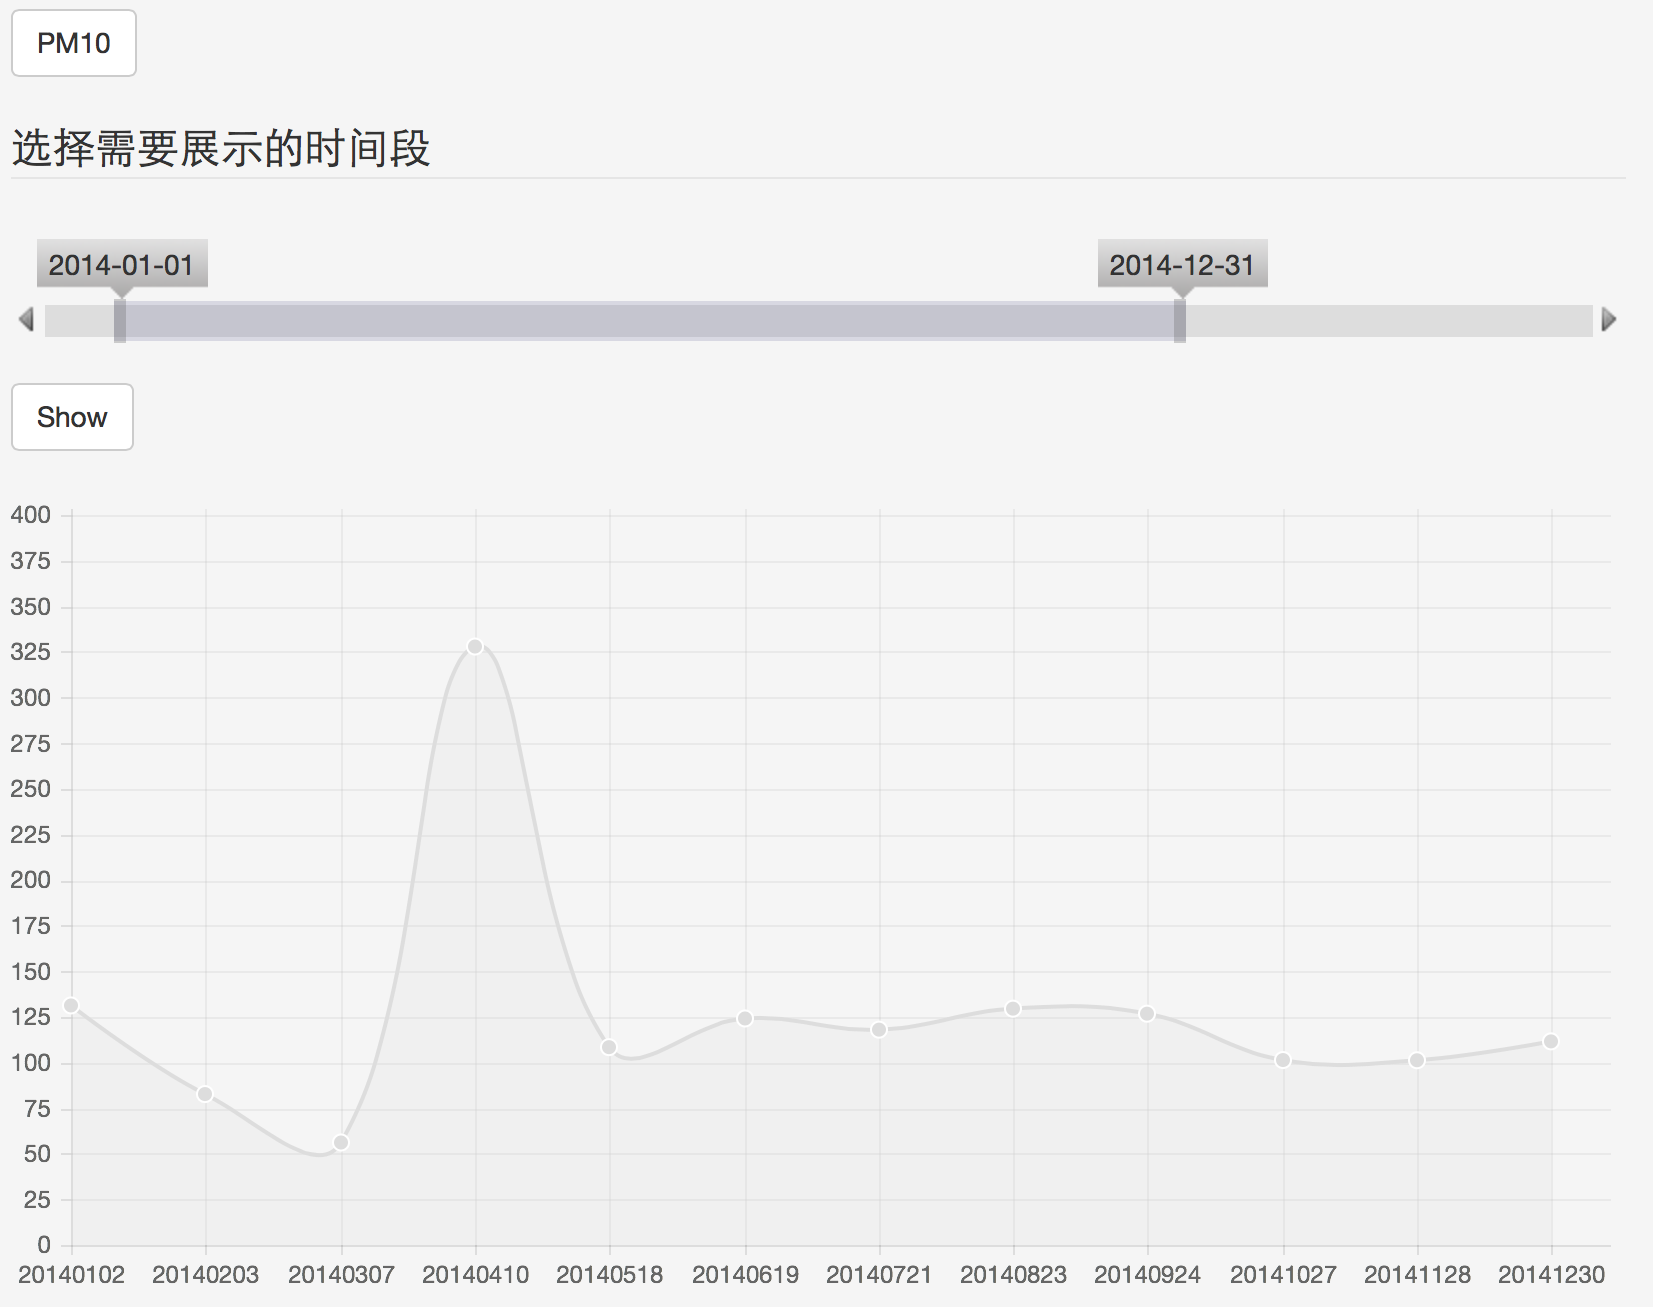
\includegraphics{7.png}}
\caption{\textit{PM10全年浓度变化}}
\end{figure}

\newpage

\begin{figure}[ht]
\centering
\scalebox{0.5}{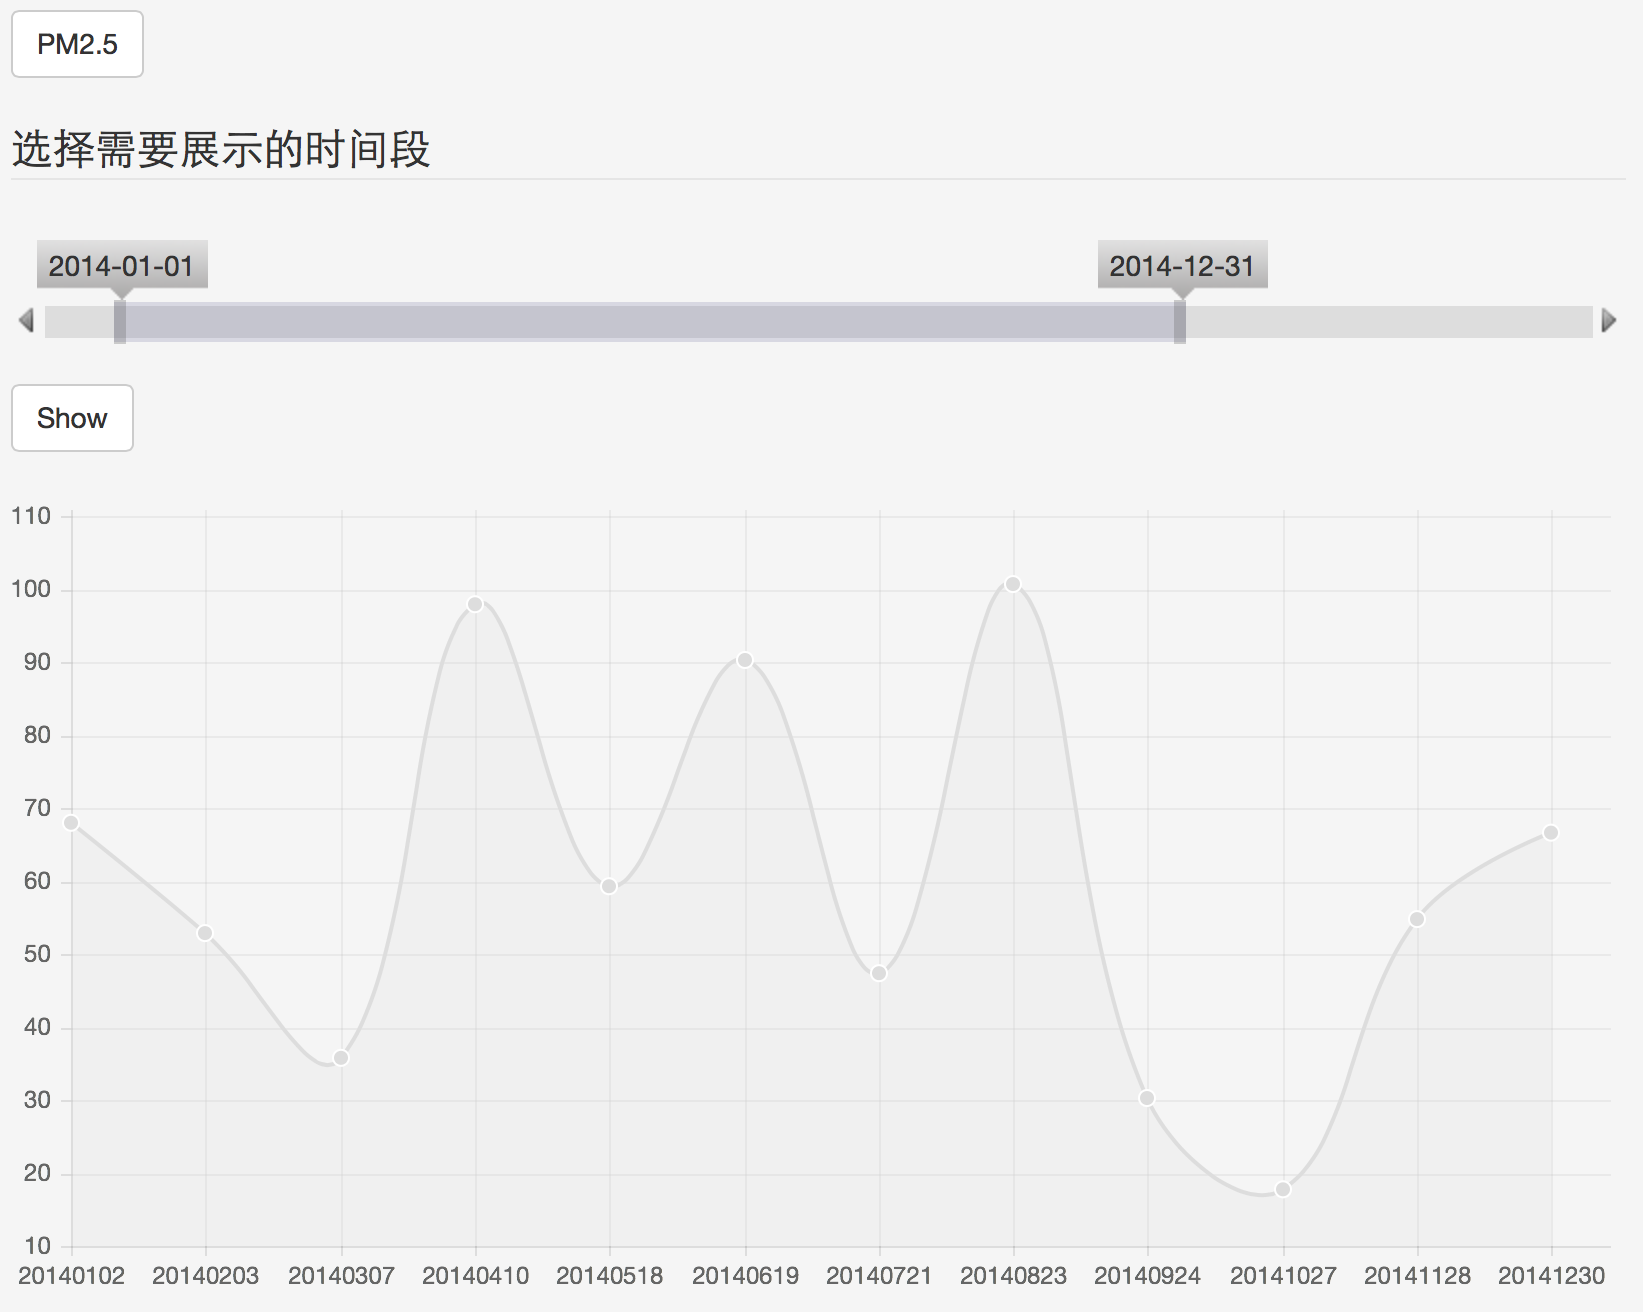
\includegraphics{8.png}}
\caption{\textit{PM2.5全年浓度变化}}
\end{figure}

\subsection{APEC会议期间空气质量}
\qquad APEC会议时间是2014年11月5日至11日,华北地区全面减排是从11月3号开始的,这个月北京的PM2.5浓度变化如下。除了11月9日浓度稍有上升以外,整个会议期间空气质量都是很好的。而会议结束后空气质量的明显变差也提醒了我们,空气质量也是可防可控的。

\begin{figure}[ht]
\centering
\scalebox{0.5}{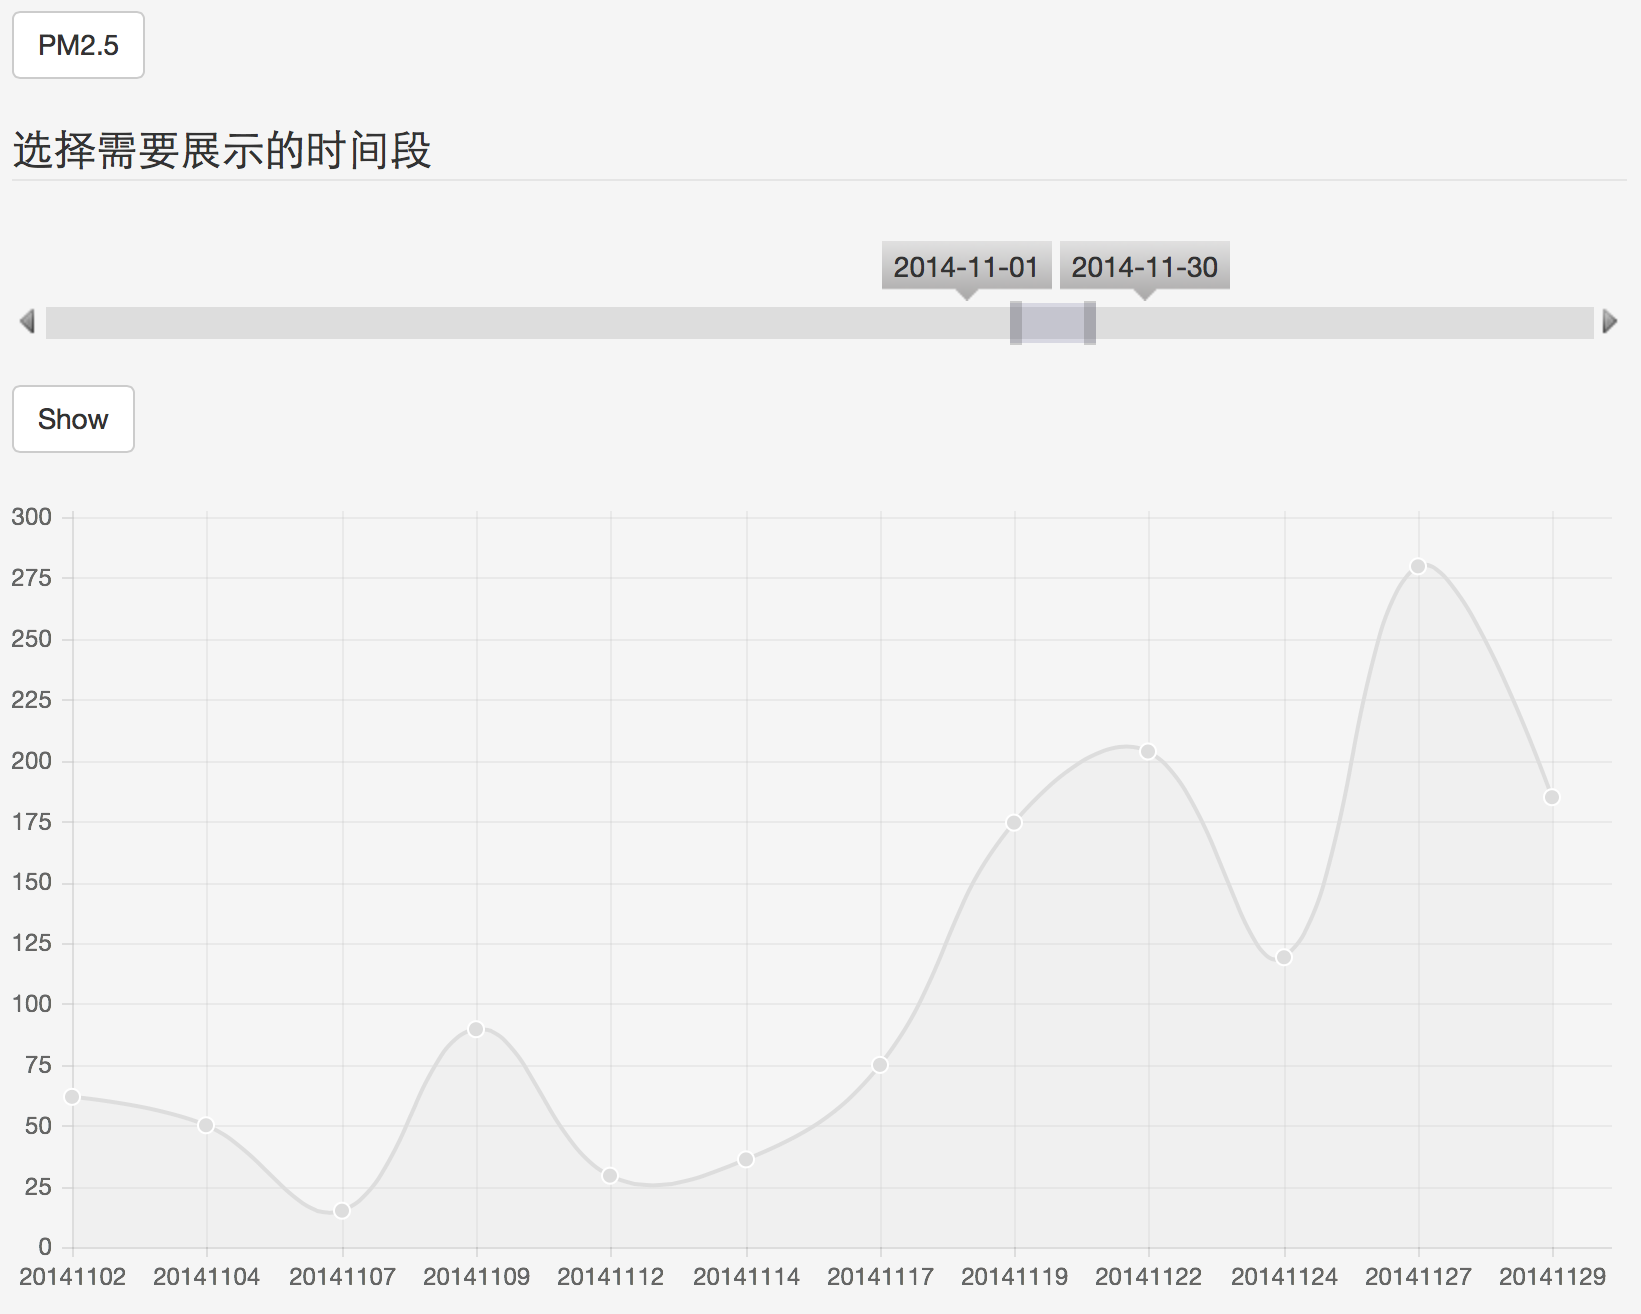
\includegraphics{9.png}}
\caption{\textit{APEC会议期间空气质量}}
\end{figure}

\subsection{冬季供暖的影响}
\qquad 北京供暖期是每年的11月15日至次年的3月15日,一共4个月,为了进行对比,把这个时间段扩展一倍,即前延到9月15日,后延到5月15日,考察这段时间的$PM_{2.5}$ 浓度。可以看到,除了APEC会议期间,供暖期的空气质量是明显糟于其余时段的。

\begin{figure}[ht]
\centering
\scalebox{0.5}{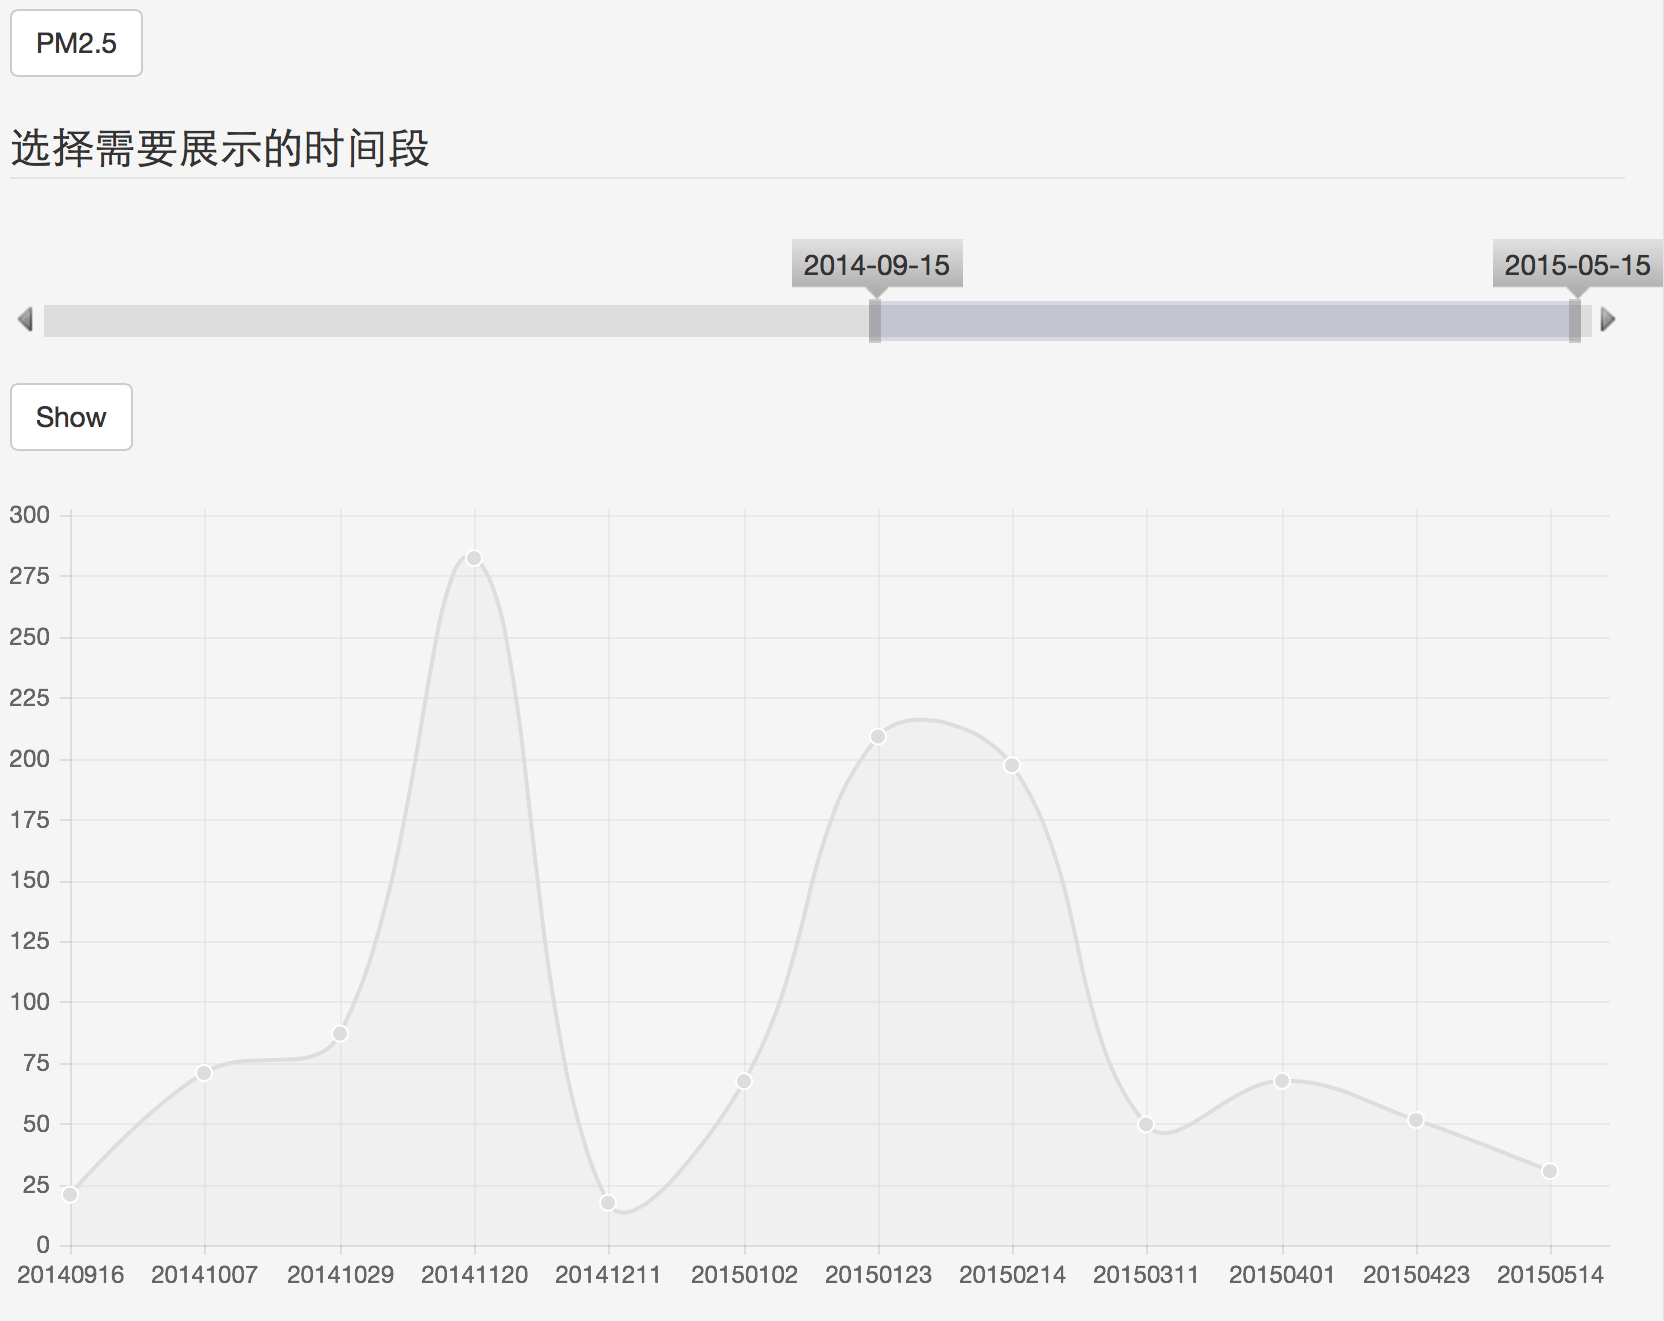
\includegraphics{10.png}}
\caption{\textit{冬季供暖对空气质量的影响}}
\end{figure}


\subsection{年度之间的变化}
\qquad 受数据时间范围的限制(仅拥有2013年12月至2015年6月的数据),所以只对2013年12月和2014年12月的空气质量进行了对比。注意到2013年图中的纵轴坐标与2014年中的不同,整体曲线形状也证明了2014年空气质量优于2013年,这也是一个可喜的结果。

\begin{figure}[ht]
\centering
\scalebox{0.5}{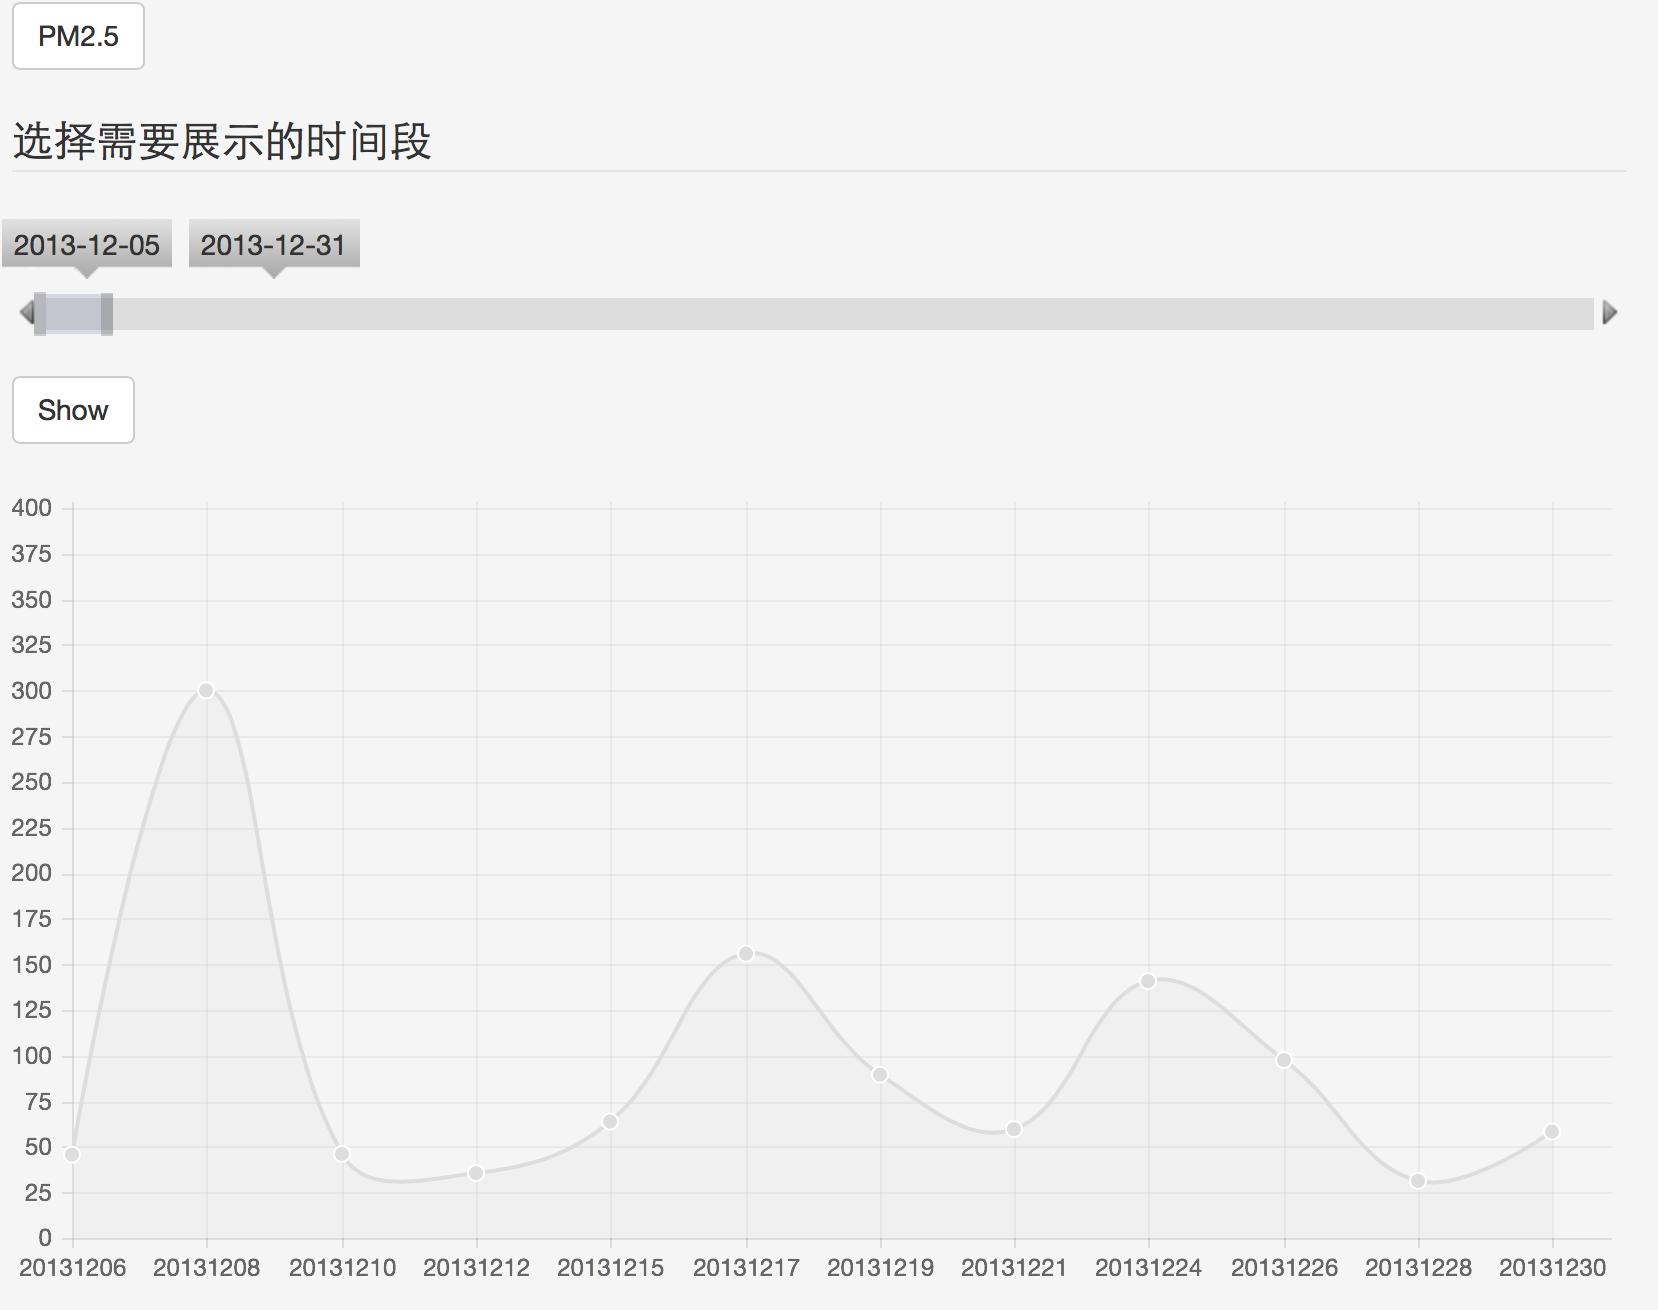
\includegraphics{11.png}}
\caption{\textit{2013年12月空气质量}}
\end{figure}

\begin{figure}[ht]
\centering
\scalebox{0.5}{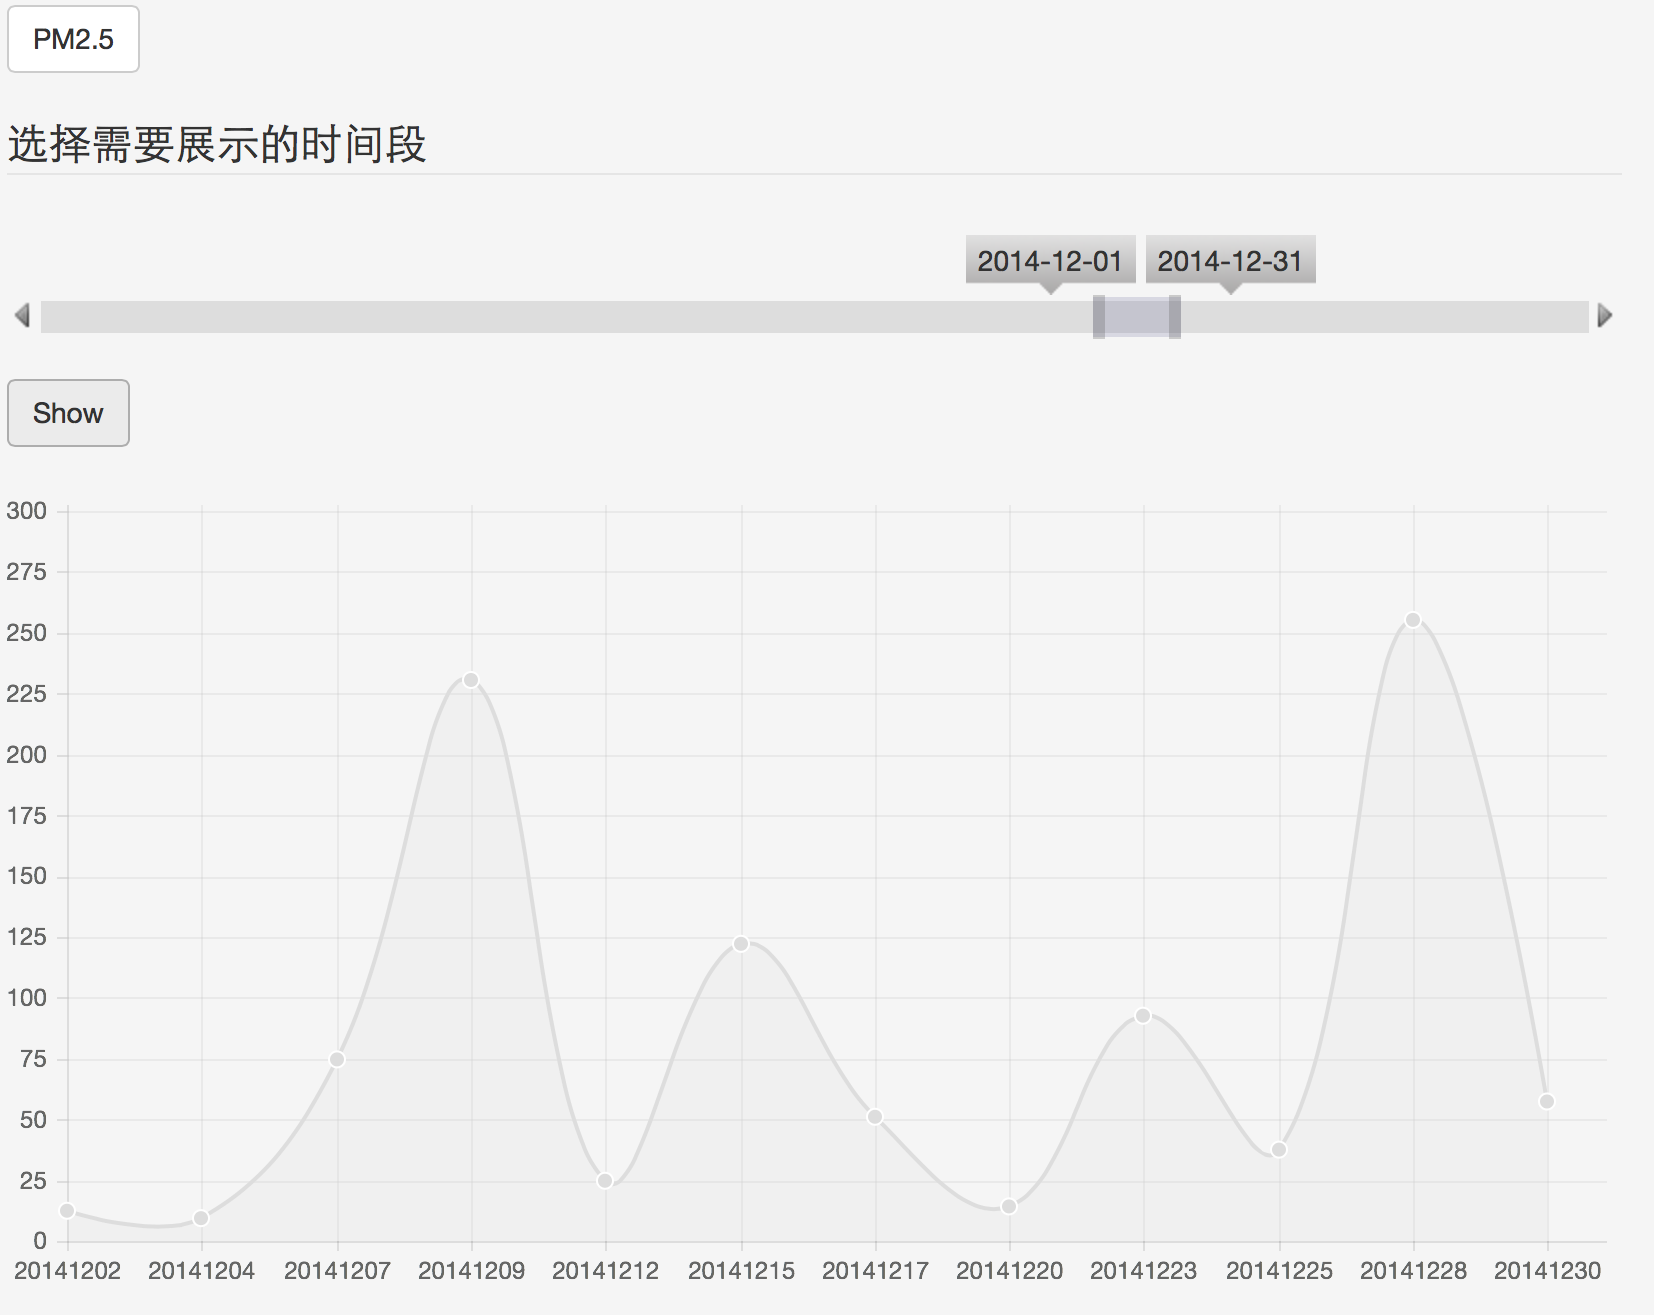
\includegraphics{12.png}}
\caption{\textit{2014年12月空气质量}}
\end{figure}

\end{CJK*}
\end{document}
